\documentclass[a4paper,11pt]{article}

% --- Typography & Page Geometry ---
\usepackage[english]{babel}
\usepackage{lmodern}
\usepackage[T1]{fontenc}
\usepackage[utf8]{inputenc}

\usepackage[margin=2.5cm]{geometry}
\usepackage{microtype}
% --- Math Formatting & Spacing ---
\usepackage{amsmath,amssymb,amsthm}
\usepackage{mathtools}
\usepackage{bbm}
\usepackage{stmaryrd}

% Math theorem spacing customization
\newtheoremstyle{spaced}
  {8pt} % Space above
  {8pt} % Space below
  {\itshape} % Body font
  {}    % Indent amount
  {\bfseries} % Theorem head font
  {.}   % Punctuation after theorem head
  {.5em}% Space after theorem head
  {}    % Theorem head spec
\theoremstyle{spaced}
\newtheorem{definition}{Definition}
\newtheorem{theorem}{Theorem}

% --- Graphics, Algorithms & Tables ---
\usepackage{graphicx}
\usepackage{subcaption}
\usepackage{algorithm}
\usepackage{algpseudocodex}

\usepackage{booktabs, tabularx}
\AtBeginDocument{
  \renewcommand{\arraystretch}{1.2} % Gives table rows slight breathing room
}

% --- Boxes & Links ---
\usepackage{tcolorbox}
\tcbuselibrary{skins, breakable}
% Global styling for tcolorbox to avoid tight defaults
\tcbset{
  before skip=10pt,
  after skip=10pt,
  boxsep=3pt,
  top=6pt, bottom=6pt, left=8pt, right=8pt
}

\usepackage{url}

% --- Paragraph Spacing ---
\usepackage{parskip} % Adds vertical space between paragraphs, eliminates manual \noindent


\usepackage{hyperref}
\hypersetup{
    colorlinks=true,
    linkcolor=blue,
    citecolor=blue,
    urlcolor=blue,
    pdftitle={RL\&NSAI},
    pdfauthor={Dancelli Elia},
    pdfcreator={\LaTeX{} with \flqq hyperref \frqq package},
}
\usepackage{soul}
\usepackage{geometry}
\geometry{margin=2.5cm}

\usepackage{tikz}
\usetikzlibrary{arrows.meta, positioning}

\DeclareMathOperator*{\argmax}{argmax}
\DeclareMathOperator*{\argmin}{argmin}

\begin{document}

\begin{titlepage}
    \centering

    \vspace*{3cm}

    {\Huge \bfseries Reinforcement Learning \& Neurosymbolic AI\par}
    \vspace{0.4cm}
    {\Large Summary of Lesson's Notes of A.Y. 25 -- 26 course\par}

    \vfill

    \begin{flushleft}
        \textsc{Dancelli Elia}\\
    \end{flushleft}

    \vspace{1cm}

    \begin{flushright}
        \textbf{Last updated}\\
        \today
    \end{flushright}

\end{titlepage}

\section*{Attribution and Licensing Notice}

These lecture notes incorporate material, concepts, and structure adapted from the following open educational resources:

\begin{itemize}
    \item \textbf{David Silver's Reinforcement Learning Course (UCL):} 
    Course materials, slides, and lecture content by David Silver. 
    Licensed under the \href{https://creativecommons.org/licenses/by-nc/4.0/}{Creative Commons Attribution-NonCommercial 4.0 International License (CC BY-NC 4.0)}. Third-party content contained therein is excluded from this license.
    
    \item \textbf{Reinforcement Learning: An Introduction (2nd Edition):} 
    By Richard S. Sutton and Andrew G. Barto (The MIT Press). 
    Licensed under the \href{https://creativecommons.org/licenses/by-nc-nd/2.0/}{Creative Commons Attribution-NonCommercial-NoDerivs 2.0 Generic License (CC BY-NC-ND 2.0)}.
\end{itemize}

\vspace{0.5cm}
\noindent
\textbf{Usage Restrictions:} This document is made available for non-commercial educational and personal study purposes only, in compliance with the CC BY-NC licenses of the source materials.

\clearpage

\tableofcontents

\newpage

\section{Introduction}
\subsection{What's Reinforcement Learning?}

To us \textbf{intelligence} is the fact to be able to make decisions and to achieve goals. In general people and animals learn by interacting actively with the environment: this type of learning is:
\begin{itemize}
    \item \textbf{Active}
    \item \textbf{Sequential:} future interactions depend on earlier ones
    \item \textbf{Goal-directed}
\end{itemize}


The goal is to optimize the sum of rewards, through repeated interactions with the environment around us.

\begin{definition}[Reward]
    A \textbf{reward} is a scalar feedback signal, which tells us information about the immediate performance at time step $t$
\end{definition}

\begin{definition}[Reward Hypothesis]
    Any goal can be formalized as the outcome of maximizing a cumulative reward
\end{definition}

\subsection{Agent and Environment}
An agent is fully described by its state at a certain time $t$, which is defined from the observation at time $t$.  The agent state $S$ is a function of the \textbf{history}, e.g. the full sequence of $observation \to actions \to rewards$.

\[
    H_t = O_0, A_0, R_0, O_1, \dots, O_{t-1}, A_{t-1}, R_t, O_t
\]

Formally the state $S_t$ at a certain time-step $t$ is a function of the history $S_t = f(H_t)$

The agent state at timestep $t+1$ can be described by:
\[
    S_{t+1} = u(S_t, A_t, R_{t+1}, O_{t+1})
\]
where $u$ is called the \textbf{state update function}. But one may ask: why bother with $u$ at all? In general the agent doesn't get to see the true environment state, but only an observation $O_t$. The update function $u$ is the agent's own bookkeeping: a way of compressing everything it has seen so far into a summary that is (ideally) Markovian, even when the raw observations aren't. When $S_t = O_t$ (full observability), $u$ is trivial ($u(S_t, A_t, R_{t+1}, O_{t+1}) = O_t$); when it isn't, $u$ is doing real work.

At each step $t$ the agent:
\begin{itemize}
    \item Receives observation $O_t$ and reward $R_t$
    \item Executes action $A_t$
\end{itemize}

\begin{center}
    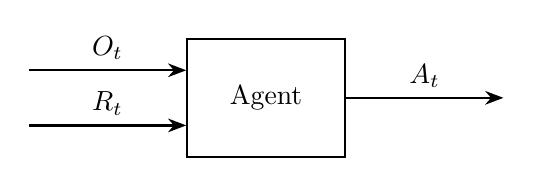
\begin{tikzpicture}[
        agent_box/.style={
            draw, 
            rectangle, 
            minimum width=2cm, 
            minimum height=1.5cm, 
            thick
        },
        arrow_style/.style={
            ->, 
            >=Stealth, 
            thick
        }
    ]
        \node[agent_box] (agent) {Agent};
        \coordinate[left=2cm of agent.west, yshift=0.35cm] (in_O);    
        \coordinate[left=2cm of agent.west, yshift=-0.35cm] (in_R);
        \coordinate[right=2cm of agent.east] (out_A);
        \draw[arrow_style] (in_O) -- node[above] {$O_t$} (agent.west |- in_O);
        \draw[arrow_style] (in_R) -- node[above] {$R_t$} (agent.west |- in_R);
        \draw[arrow_style] (agent.east) -- node[above] {$A_t$} (out_A);
    \end{tikzpicture}
\end{center}

The environment state $S_t^e$ is the environment's internal "private" representation, which may be very complicated, especially for real world environments. This is usually invisible to the agent. The \textbf{agent state} $S_t^a$, instead, is the agent's internal representation, i.e. whatever information the agent uses to pick the next action.
The environment:
\begin{itemize}
    \item Receives the action $A_t$
    \item Emits observation $O_{t+1}$ and reward $R_{t+1}$
\end{itemize}

\noindent
\textbf{Note:} when the agent sees the full environment state we talk about \textit{full observability} ($S_t = O_t$)

\noindent
The objective of the agent is to \textbf{maximize cumulative reward}
\[
    G_t = R_{t+1} + R_{t+2} + R_{t+3} + \dots
\]

Where $G_t$ is called \textbf{return}. Note that it refers to the \textit{future} and not to the past!

\subsubsection{Values}
\begin{tcolorbox}[colframe=black, coltitle=white, title=Note, fonttitle=\bfseries]Since RL environments are often \textit{stochastic}, we can't predict exactly what will happen, that's why we use the \textbf{expected value} $\mathbb{E}$, which represents the average outcome over many possible futures.
\end{tcolorbox}

We call the \textbf{expected cumulative reward} from a state $a$, the value:
\begin{align*}
    v(s) &= \mathbb{E}[G_t \mid S_t = s] \\
         &= \mathbb{E}[R_{t+1} + R_{t+2} + \dots \mid S_t=s]
\end{align*}

This can be thought as the \textit{long-term potential} of being in a specific state. While a reward tells you how good your last action was, the value tells you how good your long-term future looks from where you are standing. The goal is to maximize this value by picking the most "useful" states and actions. In general returns and values can be defined recursively:
\begin{align*}
    G_t &= R_{t+1} + G_{t+1} \\
    v(s) &= \mathbb{E}[R_{t+1} + v(S_{t+1}) \mid S_t = s]
\end{align*}

\noindent
Sometimes it might be better to sacrifice immediate reward to gain more long-term reward
\begin{itemize}
    \item Refueling a helicopter might prevent a crash in several hours
    \item Learning a new skill can be costly and time-consuming at first
\end{itemize}

It is also possible to condition the value on the actions taken
\begin{align*}
    q(s,a) &= \mathbb{E}[G_t \mid S_t=s, A_t = a] \\
            &= \mathbb{E}[R_{t+1}+ R_{t+2} + \dots \mid S_t = s, A_t = a]
\end{align*}

\subsection{Policy}
A \textbf{policy} $\pi(\cdot)$ defines the agent's behaviour and can be roughly described as a mapping from the agent state to action $a \sim \pi(s)$

There are two kinds of policies:
\begin{itemize}
    \item \textbf{Deterministic} $A=\pi(S)$, we always take the same action in a given state
    \item \textbf{Stochastic} 
    \begin{align*}
        &\pi : S \times A \to [0,1], \qquad \text{with } \sum_{a \in \mathcal{A}} \pi(s,a) = 1 \ \ \forall s \in \mathcal{S} \\
        &\pi(a \mid s) = p(A_t=a \mid S_t = s)
    \end{align*}
\end{itemize}

We will write this equivalently as $\pi(a \mid s)$, i.e. $\pi(s,a) = \pi(a \mid s)$, and use the conditional notation from here on.

\subsubsection{Value function}
The value functions provide information about the objective. They help an agent
understand how good the states and available actions are in terms of the expected future
return. The actual value function is expressed as
\begin{align*}
    v_\pi(s) &= \mathbb{E}_\pi[G_t \, | \, S_t=s] \\
             &= \mathbb{E}_\pi[R_{t+1}+\gamma R_{t+2} + \gamma^2 R_{t+3} +\dots \, | \, S_t=s]
\end{align*}
Here we introduced the so-called \textbf{discount factor} $\gamma \in [0,1]$. Even the discounted return has a recursive form:
\begin{align*}
    G_t &= R_{t+1}+\gamma R_{t+2} + \gamma^2 R_{t+3} + \dots \\
                  &= R_{t+1}+\gamma(\underbrace{R_{t+2} + \gamma R_{t+3} +\dots}_{G_{t+1}} ) \\
                  &= R_{t+1} + \gamma G_{t+1}
\end{align*}
Therefore, the value has a recursive definition as well:
\begin{align*}
    v_\pi(s) &= \mathbb{E}_\pi[R_{t+1} + \gamma G_{t+1} \, | \, S_t=s] \\
             &= \mathbb{E}_\pi[R_{t+1} + \gamma v_\pi(S_{t+1}) \, | \, S_t=s]
\end{align*}
This is known as the \textbf{Bellman equation} and a similar equation holds for the optimal value $v_\star(s)$ and $q_\star(s,a)$:
\begin{align*}
    v_\star(s) &= \max_{a} \mathbb{E}[R_{t+1}+\gamma v_\star(S_{t+1}) \, | \, S_t = s, \mathcal{A}_t = a]\\
    q_\star(s,a) &= \mathbb{E}\!\left[R_{t+1} + \gamma \max_{a'} q_\star(S_{t+1}, a') \,\middle|\, S_t = s, A_t = a\right]
\end{align*}

Note that this equation \textbf{does not} depend on a policy.


\subsection{Markov Decision Processes}

\begin{definition}[Markov Process]
    A decision process is called a \textbf{markov process} if
    \[
        p(s',r \mid S_t, A_t) = p(s', r \mid H_t, A_t)
    \]
    where
    \begin{itemize}
        \item $s'$ is the next state
        \item r is the reward obtained in s
    \end{itemize}
\end{definition}

Essentially this means that the state contains everything we need to know from the history, so that adding more history does not help.

\subsection{Model}\label{sec:model}
A \textbf{model} predicts what the environment will do next, e.g. $\mathcal{P}$ that predicts the next state:
\[
    \mathcal{P}(s,a,s') \approx p(S_{t+1}=s' \mid S_t = s, A_t = a)
\]
or $\mathcal{R}$ that predicts the next reward:
\[
    \mathcal{R}(s,a) \approx \mathbb{E}[R_{t+1} \mid S_t=s, A_t=a]
\]


\section{Exploration vs. Exploitation}
Learning agents needs to trade off two things:
\begin{itemize}
    \item \textbf{Exploration:} increase the amount of knowledge
    \item \textbf{Exploitation:} maximize the performance based on current knowledge
\end{itemize}

\subsection{K-armed Bandit}
Consider the following learning problem. You are faced repeatedly with a choice among $k$ options, or actions. After each choice you receive a numerical reward chosen from a stationary probability distribution that depends on the action you selected. Your objective is to maximize the expected total reward over some period, for example, over 1000 actions selections, or \textit{time steps}.
\begin{itemize}
    \item The original problem was named by an analogy to a slot machines with $k$ levers, where each action is like a play of one of the slot machine's levers and the rewards are the payoffs for hitting the jackpot.
\end{itemize}

\subsubsection{Greedy algorithms}\label{lab:greedy_algorithms}

In our problem each of the $k$ actions has an expected/mean reward given that that action is selected; let us call this the \textbf{value} of that action. The value of an arbitrary action $a$, denoted $q_\star (a)$, is the expected reward, given that $a$ is selected:
\[ 
    q_\star (a) = \mathbb{E}[R_t \mid A_t=a]
\]

We assume that we do not know the action values with certainty, although we have the estimated value of action $a$ at time step $t$, denoted as $Q_t(a)$. We'd like $Q_t(a)$ to be as close as possible to $q_\star (a)$. If we maintain estimates of the action values, then at any time step there is at least one action whose estimated value is greatest: we call these the \emph{greedy} actions. When we select one of these actions, we say that we are \textbf{exploiting} the current knowledge of the value of the actions. If, instead, we select one of the non-greedy actions then we say we are \textbf{exploring}, because this enables to improve the estimate of the non-greedy action values.


Recall that the true value of an action is the mean reward when that action is selected. A simple estimate of this quantity is the following:
\[  
    Q_t(a) = \frac{\text{sum of rewards when $a$ taken prior to $t$}}{\text{number of times $a$ taken prior to $t$}} = \frac{\sum_{i=1}^{t-1} R_i \cdot \mathbbm{1}(A_i=a)}{\sum_{i=1}^{t-1} \mathbbm{1}({A_i=a})}
\]

Where $\mathbbm{1}(predicate)$ denotes the random variable that is 1 if $predicate$ is true and 0 if it is not. Here the simplest action selection rule is to select one of the actions with the highest estimated value:
\[
    A_t = \argmax_{a} Q_t(a)
\]

That is a \textbf{greedy} action selection, that always exploits current knowledge to maximize immediate reward. Note the greediness stops the algorithm from sampling apparently inferior actions to see if they might really be better! That's why $\varepsilon$-$greedy$ methods got introduced: with a small probability $\varepsilon$ we select the action randomly from among the all possible actions. In the remaining cases we use normal greedy action selection.

\subsubsection{Gradient bandits}
Now the question is: can we learn policies $\pi(a)$ directly, instead of learning values? For instance, let's define an \textbf{action preference} function $H_t(a) \in \mathbb{R}$, a sort of "liking" for a certain action $a$. To turn these abstract preferences into actual probabilities, we use the \textbf{Softmax} distribution:
\[
    p(A_t=a) = \pi_t(a) = \frac{e^{H_t(a)}}{\sum_{b} e^{H_t(b)}}
\]
Where $\pi_t(a)$ represents the probability of taking action $a$ at time $t$.
That's all good, but now how do we learn these preferences? Since we aren't just averaging rewards anymore, we update $H_t(a)$ using \textbf{Stochastic Gradient Ascent}. We now define the performance of our policy $\pi_\theta$ as the expected reward we get when following it. We call this $J(\theta)$: 

\[
    J(\theta) \doteq \mathbb{E}[R_t \mid \pi_\theta] = \sum_a \pi_\theta(a) \cdot q_\star(a)
\]
Our goal is to find the parameters $\theta$ (in our case, the preferences $H_t(a)$) that make $J(\theta)$ as large as possible. Since we want to maximize $J(\theta)$, we move our parameters in the direction that increases the expected reward most steeply. This direction is the \textbf{gradient}:
\[
    \theta_{t+1} = \theta_t + \alpha \nabla_\theta \mathbb{E}[R_t \, | \, \pi_{\theta_t}]
\]
Where:
\begin{itemize}
    \item $\theta_t$: our current internal preferences.
    \item $\alpha$: the step size
\end{itemize}

Now we would like to have $\nabla_\theta \mathbb{E}[R_t \mid\pi_\theta]$, but there's a problem: the expectation is over actions sampled from $\pi_\theta$, and $\theta$ lives inside that distribution, and we can't just push the gradient through a sampling operation the way we would with a normal function. The \textbf{log-likelihood trick} (also called REINFORCE) is the standard fix to this issue: it rewrites the gradient of an expectation as an expectation of a gradient

\[
    \nabla_\theta \mathbb{E}[R_t \mid \pi_\theta] = \mathbb{E}[R_t \nabla_\theta \ln (\pi_\theta(a))]
\]
Now, we need to find $\nabla_\theta \ln \pi_\theta(a)$ specifically for the Softmax function. In our case, the parameters $\theta = H_t(a)$. We need to calculate how the log-probability of an action a changes when we nudge a specific preference $H_t(k)$. Taking the partial derivative of the softmax gives us two different scenarios:
\begin{equation}
    \frac{\partial \ln \pi_t(a)}{\partial H_t(k)} = 
    \begin{cases} 
        1 - \pi_t(a) & \text{if } k = a \\
        -\pi_t(k)    & \text{if } k \neq a 
    \end{cases}
\end{equation}


\noindent
There is a natural learning algorithm for softmax action preferences based on the idea of stochastic gradient ascent. On each step, after selecting action $A_t$ and receiving the reward $R_t$, the action preferences are updated by:
\begin{equation}
    H_{t+1}(a) =
    \begin{cases}
        H_t(a) + \alpha R_t \cdot (1 - \pi_t(a)) &\qquad \text{if } a=A_t \\
        H_t(a) - \alpha R_t \cdot \pi_t(a) &\qquad \text{if } a \neq A_t
    \end{cases}
\end{equation}
This update mechanism creates a "push-pull" effect that ensures the policy remains a valid probability distribution:
\begin{itemize}
    \item For the chosen action $a=A_t$ we "push up" the preference. The term $(1-\pi_t(a))$ acts as a scaling factor, so that if the action was already likely the update is small, else the update is much larger
    \item For all other actions $a \neq A_t$ we "pull down" the preferences by subtracting $\alpha R_t \pi_t(a)$, we ensure that as one action becomes more desirable, the others become relatively less likely, maintaining the balance of the softmax distribution.
\end{itemize}
Now let's imagine what happens if our rewards $R_t$ are large and positive: then the basic update will push all action preferences up significantly, even for the "bad" actions. The model eventually figures it out, but it's a slow, noisy process. The solution is to introduce a so-called \textbf{baseline} $b$ to the gradient-ascent rule update:

\[
    \theta_{t+1} = \theta_t + \alpha (R_t - b) \nabla_\theta \ln \pi_\theta (A_t)
\]

Mathematically everything works out as expected, since adding the baseline does not change the expected update:

$$\mathbb{E}_{a\sim\pi_\theta}\big[b\,\nabla_\theta \ln \pi_\theta(a)\big] =
b\sum_a \nabla_\theta \pi_\theta(a) = b\,\nabla_\theta\sum_a \pi_\theta(a) = b\,\nabla_\theta(1) = 0$$

since $b$ doesn't depend on the action being summed over, and probabilities always sum to $1$

\subsection{How well can we do?}
While the Policy Gradient method with a baseline helps us converge faster, the Lai \& Robbins Theorem (1985) reminds us that exploration has a mandatory cost. Lai \& Robbins proved that for any reasonable strategy, the total regret must grow at least \textbf{logarithmically} with the number of steps $t$. Before going into the conclusion, we need to introduce some other concept needed for understanding it. First, let's remind ourselves what $q_\star$ is:

\[
    q_\star = \max_{a \in A} q(a) = \max_{a} \mathbb{E}[R_t \mid A_t = a]
\]
which is the \textbf{optimal value} achievable by any single action in the current environment. Instead, we call $q_\star(a)$ the \textbf{true value} (e.g. the expected reward) of a specific action $a$. We then define the \textbf{regret} of taking an action as:

\[
    \Delta_a \doteq q_\star - q_\star(a) 
\]
In other words, the regret represents the gap between the best action possible and the action $a$ which was actually chosen. The last piece we need to introduce is the \textbf{total regret} which, you can imagine, is the sum of all the single regrets:

\[
    L_t = \sum_{n=1}^{t} \left( q_\star - q(A_n) \right) = \sum_{n=1}^t \Delta_{A_n}
\]

Before stating Lai \& Robbins' result we need one tool from information theory: a way to measure "how different" two probability distribution are and that's exactly what KL divergence gives us. Intuitively: if pulling arm $a$ and pulling the optimal arm produce reward distributions that look almost identical, no amount of data will let you tell them apart quickly — you're forced to keep sampling the suboptimal arm just to gather enough evidence. That "forced sampling cost" is exactly what shows up as $1/D_{KL}$ in the regret bound below: small KL divergence $\Rightarrow$ big minimum regret.

\begin{definition}[Kullback-Leibler Divergence]
    The \textbf{Kullback-Leibler divergence} $D_{KL}(p \parallel q)$ is a measure from information theory that quantifies how much one probability distribution $p$ deviates from a second reference probability distribution $q$

    \[
        D_{KL}(p \parallel q) = \sum_{x \in \mathcal{X}} p(x) \log \frac{p(x)}{q(x)}
    \]
\end{definition}

\begin{theorem}[Lai \& Robbins]
    The asymptotic total regret is \textbf{at least logarithmic} in the number of steps $t$
    \[
        \liminf_{t\to\infty} \frac{L_t}{\ln t} \;\ge\; \sum_{a:\Delta_a>0} \frac{\Delta_a}{D_{KL}(p_a \,\|\, p_\star)}
    \]
\end{theorem}

\noindent
Let's dive into the formula a bit more:
\begin{itemize}
    \item We are summing over all $\Delta_a > 0$, that means we are summing over all suboptimal actions
    \item The Kullback-Leibler divergence measures how distinct the reward distribution $p_a$ is from the reward distribution given by choosing the best action $p_\star$.
    \begin{itemize}
        \item If $D_{KL}$ is high, that means that the actions we took are far from the optimal ones
        \item If, instead, $D_{KL}$ is low, that means that the distributions are very similar.
    \end{itemize}
    Note a thing: when the denominator $D_{KL}$ is small, the total regret goes up. This means you are forced to pull that suboptimal arm many times just to gather enough statistical evidence to prove it is actually worse than the best arm.
\end{itemize}

\subsection{Upper-Confidence-Bound action selection}
As we saw in section (\ref{lab:greedy_algorithms}), $\varepsilon$-greedy action selection forces the agent to explore, but it does so indiscriminately, with no preference for nearly-greedy actions or particularly uncertain actions. It would be better to favor non-greedy actions according to their potential for actually being optimal, taking into account how close their estimates are to being maximal and the uncertainties in those estimates. One effective way of doing this is to select actions according to:

\[
    A_t \doteq \argmax_{a} \left[ Q_t(a) + c \sqrt{\frac{\ln t}{N_t(a)}}\right], \qquad N_t=\sum_i \mathbbm{1}(A_i=a)
\]

\noindent
The motifs behind the choice of this specific functional form are:
\begin{itemize}
    \item The formula explicitly splits the decision into \textit{exploitation} ($Q_t(a)$) and \textit{exploration} (the term under the square root)
    \item The term under the square root serves as an estimate of the variance. Each time an action $a$ is selected, in fact, the $N_t(a)$ term grows, lowering the overall uncertainty.
    \item Each time an action $a' \neq a$ is chosen, $t$ increases but $N_t(a)$ does not, and this makes the global uncertainty grow 
\end{itemize}

\begin{theorem}[Auer, Cesa-Bianchi, and Fischer, 2002]
    For the UCB algorithm, using $c=\sqrt{2}$, the expected total regret after $n$ steps is at most:
    \[
        L_t \leq \left[ 8 \sum_{a \mid \Delta_a > 0} \frac{\ln t}{\Delta_a} \right] + \left( 1 + \frac{\pi^2}{3}\right) \left( \sum_{j=1}^{K} \Delta_j \right)
     \]
\end{theorem}

Where $K$ is the number of machines the UCB policy is being run on.

This result is fundamental because it provides a \textbf{finite-time bound} on regret. While the Lai \& Robbins theorem was an asymptotic result (valid as $t \to \infty$), Auer et al. proved that UCB achieves \textbf{logarithmic regret} $\forall n > 0$. This confirms that UCB is not just a heuristic, but a mathematically optimal way to balance exploration and exploitation.

\section{Markov Decision Processes}
MDPs are a classical formalization of sequential decision-making, where actions influence not just immediate rewards, but also subsequent situations, or states, and through those future rewards. Whereas in bandit problems we estimated the value $q_\star(a)$ of each action $a$, in MDPs we estimate the value $q_\star(\mathbf{s},a)$ of each action $a$ in each state $s$. In fact, the $k$-armed bandit problem is just an MDP with $\lvert\mathcal{S}\rvert = 1$: there is
only one state to be in, so there is nothing to transition to, and $q_\star(s,a)$ collapses back down to $q_\star(a)$.

More intuitively: if you're in state $s$ and take action $a$, this single joint distribution tells you everything about what happens next; both which state you land in and what reward you get. This joint form is more general than treating $P$ and $R$ separately in \ref{sec:model}: that separation is really a special case that assumes reward and next-state are decoupled given $(s,a)$.

In MDPs, the random variables $R_t$ and $S_t$ have well-defined discrete probability distributions dependent only on the preceding state and action. That is, for particular values of these random variables $s' \in \mathcal{S}$ and $r \in \mathcal{R}$ there is a probability of those values occurring at time $t$, given particular values of the preceding state and action:

\begin{align*}
        p(s', r | s, a) \doteq p(S_t=s', R_t = r | S_{t-1} = s, A_{t-1} = a), \qquad \forall s', s \in \mathcal{S}, r \in \mathcal{R}, a \in \mathcal{A}
\end{align*}

In general, when we have \textit{partial observability}, the observations are \textbf{not} markovian, so using them as states would not result in a MDP. When we're in this situation we call the problem a \textbf{partially observable MDP}, in which the environment's state can still be Markovian, but the agent doesn't know it.

\subsection{Value functions}
The value function $v_\pi(s) = \mathbb{E}_\pi[G_t \mid S_t=s]$, gives us a measure of how "good" a certain state is, while the state-action value function $q_\pi(s,a) = \mathbb{E}_\pi[G_t \mid S_t=s, A_t=a]$ gives us a measure of how good or bad a certain state-action pair is. These two functions are closely connected:

\[
    v_\pi(s) = \sum_{a} \pi(a \lvert s) \cdot q_\pi(s,a) = \mathbb{E}_\pi[q_\pi(S_t,A_t) \mid S_t = s]
\]
Essentially the $v_\pi(s)$ function is the expectation over the $q$-values for all the actions $a$ available in a particular state $s$ under the policy $\pi$

\begin{definition}
    The \textbf{optimal state-value function} $v^\star(s)$ is the maximum value function over all possible policies
    \[
        v^\star(s) = \max_\pi v_\pi(s)
    \]
\end{definition}

\begin{definition}
    The \textbf{optimal action-value function} $q^\star(s,a)$ is the maximum action value function over all possible policies
    \[
        q^\star(s,a) = \max_\pi q_\pi(s,a)
    \]
\end{definition}

\begin{theorem}[Optimal Policies]
    For any Markov Decision Process:
    \begin{itemize}
        \item There exist an optimal policy $\pi^\star$ that is better than or equal to all other policies, $\pi^\star \geq \pi, \forall \pi$
        \item All optimal policies achieve the optimal value function $v_{\pi^\star}(s) = v^\star(s)$
        \item All optimal policies achieve the optimal action-value function $q_{\pi^\star}(s,a) = q^\star(s,a)$
    \end{itemize}
\end{theorem}
By maximizing over $q^\star(s,a)$ we can achieve an optimal policy:

\begin{equation}
    \pi^\star(s,a) =
    \begin{cases}
        1 \quad \text{if } a = \underset{a \in \mathcal{A}}{\mathrm{argmax}} \ q^\star(s,a) \\
        0 \quad \text{otherwise}
    \end{cases} 
\end{equation}

\section{Dynamic Programming}
Dynamic Programming (DP) refers to a collection of algorithms that can compute optimal policies, but only when given a perfect model of the environment (the MDP).
\subsection{Policy Evaluation}
The computation of the state-value function $v_\pi$ is called \textit{policy evaluation} in DP literature. Recall that, for all $s \in \mathcal{S}$:

\begin{align*}
    v_\pi(s) &\doteq \mathbb{E}_\pi[G_t \mid S_t = s] \\
             &= \mathbb{E}_\pi[R_{t+1}+\gamma G_{t+1} \mid S_t = s] \\
             &= \mathbb{E}_\pi[R_{t+1}+ \gamma v_\pi(S_{t+1}) \mid S_t = s] \\
             &= \sum_{a} \pi(a \mid s) \sum_{s',r} p(s',r \mid s,a) [r + \gamma v_\pi(s')]
\end{align*}
The existence and uniqueness of $v_\pi$ are guaranteed as long as $\gamma < 1$.

\begin{algorithm}
    \caption{Iterative policy evaluation}
    \begin{algorithmic}[1]
        \State $v_0 \gets 0$ for all states
        \Repeat
        \State $\Delta \gets 0$
        \For{each $s \in \mathcal{S}$}
            \State $v_{old} \gets v(s)$
            \State $v(s) \gets \sum_a \pi(a \mid s) \sum_{s',r} p(s',r \mid s,a)[r + \gamma v(s')]$
            \State $\Delta \gets \max(\Delta, |v_{old} - v(s)|)$
        \EndFor
    \Until{$\Delta < \theta$}
    \end{algorithmic}
    \end{algorithm}

\subsection{Policy improvement}
We calculate the value function for a certain policy to find better policies: but what if from some state $s$ we'd like to know whether to change the policy to choose an action $a \neq \pi(s)$, that is an action $a$ that does not follow the current policy? One way to answer this question is to consider selecting $a$ in $s$ and thereafter following the existing policy, $\pi$.

\begin{align*}
    q_\pi(s,a) &\doteq \mathbb{E}[R_{t+1} + \gamma v_\pi(S_{t+1}) \mid S_t=s, A_t = a] \\
               &= \sum_{s',r} p(s',r \mid s,a) \left[r + \gamma v_\pi(s') \right]
\end{align*}

Now we ask ourselves: is this greater than or less than $v_\pi(s)$? If it is greater -- that
is, if it is better to select $a$ once in $s$ and thereafter follow $\pi$ than it would be to follow
$\pi$ all the time -- then one would expect it to be better still to select $a$ every time $s$ is
encountered, and that the new policy would in fact be a better one overall.

Let $\pi$ and $\pi'$ be any pair of deterministic policies such that, for all $s \in \mathcal{S}$:
\[
    q_\pi(s, \pi'(s)) \geq v_\pi(s)
\]

Then the policy $\pi'$ must be as good as, or better than, $\pi$. That is, it must obtain greater or equal expected return from all states $s \in \mathcal{S}$

\[
    v_{\pi'}(s) \geq v_\pi(s)
\]

If we have two policies $\pi$ and $\pi'$ that are identical except in state $s$ where $\pi'(s) = a \neq \pi(s)$ we can say that for states other than $s$, $q_\pi(s, \pi'(s)) \geq v_\pi(s)$ holds because the two sides are equal. Thus if $q_\pi(s,a=\pi'(s)) > v_\pi(s)$, then the changed policy is indeed better than $\pi$.


Now we can actually extend this concept of evaluating a change in the policy in a single state to evaluating changes in \emph{all} states, selecting at each state the action that appears best according to $q_\pi(s,a)$. In other words, to consider the new \emph{greedy policy} $\pi'$, given by:

\begin{align*}
    \pi'(s) &\doteq \argmax_a q_\pi(s,a) \\
            &= \argmax_a \mathbb{E}[R_{t+1} + \gamma v_\pi(S_{t+1}) \mid S_t = s, A_t = a] \\
            &= \argmax_a \sum_{s', r} p(s', r \mid s, a) [r+\gamma v_\pi(s')]
\end{align*}

\subsection{Policy iteration}
Once a policy $\pi$ has been improved using $v_\pi$ to yield a better policy $\pi'$, we can then compute $v_{\pi'}$ and improve it again to obtain an even better $\pi''$. We can thus obtain a sequence of monotonically improving policies and value functions

\[
  \pi_0 \xrightarrow{\text{E}} v_{\pi_0} 
        \xrightarrow{\text{I}} \pi_1 
        \xrightarrow{\text{E}} v_{\pi_1} 
        \xrightarrow{\text{I}} \pi_2 
        \xrightarrow{\text{E}} \dots 
        \xrightarrow{\text{I}} \pi_* 
        \xrightarrow{\text{E}} v_*
\]

where $\xrightarrow{\text{E}}$ denotes a policy \emph{evaluation} and $\xrightarrow{\text{I}}$ denotes a policy \emph{improvement}.

\begin{algorithm}
    \caption{Policy iteration for estimating $\pi \approx \pi_\star$}
    \begin{algorithmic}[1]
        \State $V(s) \in \mathbb{R}$ and $\pi(s) \in \mathcal{A}(s), \forall \, s \in \mathcal{S}$
        \Repeat \Comment{Policy evaluation}
        \State $\Delta \gets 0$
        \For{each $s \in \mathcal{S}$}
            \State $v \gets V(s)$
            \State $V(s) \gets \sum_{s',r} p(s',r \mid s, \pi(s))[r + \gamma V(s')]$
            \State $\Delta \gets \max(\Delta, |v - V(s)|)$
        \EndFor
        \Until{$\Delta < \theta$}

        \State policy-stable $\gets$ true \Comment{Policy Improvement}
        \For{\textbf{each} $s \in \mathcal{S}$}
            \State old-action $\gets \pi(s)$
            \State $ \pi(s) \gets \argmax_a \sum_{s', r} p(s', r \mid s, a) [r+\gamma V(s')]$
            \If{old-action $\neq \pi(s)$}
                \State policy-stable $\gets$ false
            \EndIf
        \EndFor

        \If{policy-stable}
            \State \Return $V \approx v_\star$ and $\pi \approx \pi_\star$
        \Else
            \State Go to line 2
        \EndIf
    \end{algorithmic}
\end{algorithm}

Note one thing: at line 6 we do not sum over all $\sum_a \pi(a \mid s)$ because we already chose the current action to execute with the current policy $\pi(s)$.

\subsubsection{Jack's Car Rental Problem}
Jack manages two locations for a nationwide car rental company. Each day, some number of customers arrive at each location to rent cars. If Jack has a car available, he rents it out and is credited \$10 by the national company. If he is out of cars at that location, then the business is lost. Cars become available for renting the day after they are returned. To help ensure that cars are available where they are needed, Jack can move them between the two locations overnight, at a cost of \$2 per car moved. We assume that the number of cars requested and returned at each location are Poisson random variables, meaning that the probability that the number is $n$ is $\frac{\lambda^n}{n!} e^{-\lambda}$, where $\lambda$ is the expected number. Suppose $\lambda$ is 3 and 4 for rental requests at the first and second locations and 3 and 2 for returns. To simplify the problem slightly, we assume that there can be no more than 20 cars at each location (any additional cars are returned to the nationwide company, and thus disappear from the problem) and a maximum of five cars can be moved from one location to the other in one night. We take the discount rate to be $\gamma = 0.9$ and formulate this as a continuing finite MDP, where the time steps are days, the state is the number of cars at each location at the end of the day, and the actions are the net numbers of cars moved between the two locations overnight.

\begin{table}[htbp]
    \centering
    \caption{MDP Formulation for Jack's Car Rental}
    \label{tab:jacks_car_rental_mdp}
    \begin{tabularx}{\textwidth}{l l X}
    \toprule
    \textbf{Component} & \textbf{Mathematical Definition} & \textbf{Domain / Details} \\
    \midrule
    \textbf{State Space ($\mathcal{S}$)} & $s = (s_1, s_2)$ & Number of cars at location 1 and location 2 at the \textbf{end of the day}. \newline $s_1, s_2 \in \{0, 1, \dots, 20\} \Rightarrow \mathbf{441 \text{ states}}$. \\
    \addlinespace
    \textbf{Action Space ($\mathcal{A}$)} & $a \in [-5, 5]$ & Net cars moved overnight from Location 1 to Location 2. \newline Positive $a$: move 1 $\to$ 2; Negative $a$: move 2 $\to$ 1. \\
    \addlinespace
    \textbf{Reward Function ($\mathcal{R}$)} & $R(s, a)$ & Expected immediate net income: \newline $\text{Revenue from rentals } (\$10/\text{car}) - \text{Moving cost } (\$2 \times |a|)$. \\
    \addlinespace
    \textbf{Discount Factor} & $\gamma = 0.9$ & Future rewards are discounted to ensure convergence over an infinite horizon. \\
    \bottomrule
    \end{tabularx}
\end{table}

\subsection{Value iteration}
One drawback to policy iteration is that each of its iterations involves policy evaluation,
which may itself be a protracted iterative computation requiring multiple sweeps through
the state set. If policy evaluation is done iteratively, then convergence exactly to $v_\pi$
occurs only in the limit: but do we actually need to converge to this value? Or we can stop earlier?

In general the policy evaluation step of policy iteration can be truncated in several ways without losing the convergence guarantees of policy iteration. One special case is when policy evaluation is stopped after just one sweep (one update of each state). This algorithm is called \emph{value iteration}:

\begin{align*}
    v_{k+1}(s) &\doteq \max_a \mathbb{E}[R_{t+1} + \gamma v_k(S_{t+1}) \mid S_t = s, A_t = a] \\
               &= \max_a \sum_{s', r} p(s', r \mid s, a) [r + \gamma v_k(s')]
\end{align*}

In policy iteration we calculate $V(s)$ for a fixed policy $\pi$, so we do not test all the possible actions, we can just use $\pi(s)$.


\begin{algorithm}
    \caption{Value iteration for estimating $\pi \approx \pi_\star$}
    \begin{algorithmic}[1]
        \Repeat
            \State $\Delta \gets 0$
            \For{\textbf{each} $s \in \mathcal{S}$}
                \State $v \gets V(s)$
                \State $V(s) \gets \max_a \sum_{s',r} p(s',r \mid s,a) [r + \gamma V(s')]$
                \State $\Delta \gets \max(\Delta, |v-V(s)|)$
            \EndFor
        \Until{$\Delta < \theta$}

        \State Output $\pi \approx \pi_\star$ such that $\pi(s) = \argmax_a \sum_{s',r}  p(s',r \mid s,a) [r + \gamma V(s')]$
    \end{algorithmic}
\end{algorithm}

Unlike policy iteration, value iteration has no separate policy being tracked during the loop -- 
$\pi$ is only extracted once, at the very end.

\begin{table}[h]
    \centering
    \caption{Policy Iteration vs.\ Value Iteration}
    \begin{tabularx}{\textwidth}{lXX}
    \toprule
     & \textbf{Policy Iteration} & \textbf{Value Iteration} \\
    \midrule
    Evaluation step & Runs to convergence (multiple sweeps) & One sweep only \\
    Update rule & Fixed-policy backup, then separate greedy improvement & $\max_a$ taken directly inside the value update \\
    Cost per outer iteration & Higher (full evaluation) & Lower (one sweep) \\
    Outer iterations needed & Fewer & More \\
    \bottomrule
    \end{tabularx}
\end{table}

\subsection{Asynchronous Dynamic Programming}
A major drawback to the DP methods is that they involve operations over the entire state set of the MDP, that is, they require sweeps of the state set. If the state set is very large, then even a single sweep can be prohibitively expensive.

\emph{Asynchronous} DP algorithms are in-place iterative DP algorithms that are not organized in terms of systematic sweeps of the state set. These algorithms update the values of states in any order whatsoever, using whatever values of other states happen to be available. The values of some states may be updated several times before the values of others are updated once. There are three main types of asynchronous programming:

\begin{enumerate}
    \item \textbf{In-place:} instead of keeping two arrays (one for the old value $V_k$ and one for new values $V_{k+1}$), we use a single array $V$.
    \item \textbf{Prioritized sweeping:} tracks which states experienced a large change in value ($\Delta V$) and prioritizes updating the predecessor states that lead into those changed states, focusing compute strictly where it makes the biggest difference
    \item \textbf{Real-time:} instead of updating random states, you run the DP update on states the agent actually encounters while interacting with the environment.
\end{enumerate}

\begin{table}[h]
    \centering
    \caption{Dynamic Programming vs.\ Monte Carlo vs.\ TD(0)}
    \begin{tabularx}{\linewidth}{l X X X}
    \toprule
     & \textbf{DP} & \textbf{MC} & \textbf{TD(0)} \\
    \midrule
    Model-free? & No & Yes & Yes \\
    Bootstraps? & Yes & No & Yes \\
    Waits for episode end? & N/A (full sweeps) & Yes & No \\
    Target & $\mathbb{E}[R + \gamma v(S')]$ & Return $G_t$ & $R + \gamma v(S')$ \\
    Bias & None & Unbiased & Biased \\
    Variance & None & High & Low \\
    Converges to & $v_\pi$ & min MSE to observed returns & max-likelihood Markov model \\
    Works in non-episodic tasks? & Yes & No & Yes \\
    \bottomrule
    \end{tabularx}
\end{table}

\section{Model-Free Prediction}
In Model-Free Prediction the objective is to estimate the value function of an \emph{unknown} MDP.

\subsection{Monte Carlo Methods}
In this section we consider our first learning methods for estimating value functions and discovering optimal policies. Here we \textbf{do not assume complete knowledge of the environment}. Monte Carlo methods require only \emph{experience} -- sequences of states, actions, and rewards from interaction with an environment.

\subsection{Monte Carlo Policy Evaluation (Prediction)}
Recall that the value of a state is the expected return starting from that state. An obvious way to estimate it from experience, then, is simply to average the returns observed after visits to that state. As more returns are observed, the average should converge to the expected value.

\begin{algorithm}
    \caption{First-visit MC prediction for estimating $V \approx v_\pi$}
    \begin{algorithmic}[1]
        \Loop
            \State Generate an episode following $\pi$: $S_0, A_0, R_1, S_1, A_1, R_2, \dots, S_{T-1}, A_{T-1}, R_T$
            \State $G \gets 0$
            \For{$t \gets T-1$ \textbf{downto} $0$}
                \State $G \gets \gamma G + R_{t+1}$
                \If{$S_t$ does not appear in $S_0, S_1, \dots, S_{t-1}$}
                    \State Append $G$ to $Returns(S_t)$
                    \State $V(S_t) \gets$ average($Returns(S_t)$)
                \EndIf
            \EndFor
        \EndLoop
    \end{algorithmic}
\end{algorithm}

When episodes are long learning can become slow because we have to wait till the end of an episode before actually learning anything useful.

\paragraph{First-visit vs.\ every-visit.} The algorithm above only records a return the
\emph{first} time a state is seen in an episode. The alternative, \emph{every-visit MC},
records a return \emph{every} time the state is visited within the same episode (so a
single episode can contribute multiple samples for the same state). Both converge to
$v_\pi$ as the number of visits $\to \infty$, but by slightly different arguments:
first-visit gives an i.i.d.\ sample of $G_t$ per episode;
every-visit samples are correlated within an episode, but the estimator is still
consistent and is more sample-efficient in practice.


\subsection{Temporal-Difference Learning}
Both TD and Monte Carlo methods use experience to solve the prediction problem. Given some experience following a policy $\pi$, both methods update their estimate $V$ of $v_\pi$. In general Monte Carlo methods
must wait until the end of the episode to determine the increment to $V(S_t)$
\[
    V(S_t) \gets V(S_t) + \alpha \left[ G_t - V(S_t) \right]
\]

Instead, TD methods need to wait only until the next time step: at time $t + 1$ they immediately form a target and make a useful update using the observed reward $R_{t+1}$ and the estimate $V (S_{t+1})$. The simplest TD method makes the update

\[
    V(S_t) \gets V(S_t) + \alpha [R_{t+1} + \gamma V(S_{t+1}) - V(S_t)]
\]

In effect, the target for the Monte Carlo update is the actual return $G_t$, whereas the target for the TD update is the estimate $R_{t+1} + \gamma V(S_{t+1})$.
\begin{itemize}
    \item $R_{t+1} + \gamma V(S_{t+1})$ is called \emph{TD Target}
    \item $\delta_t = R_{t+1} + \gamma V(S_{t+1}) - V(S_t)$ is called \emph{TD Error}
\end{itemize}

\begin{algorithm}
    \caption{Tabular TD(0) for estimating $v_\pi$}
    \begin{algorithmic}[1]
        \For{\textbf{each} episode}
            \State Initialize $S$
            \For{\textbf{each} step of episode}
                \State $A \gets$ action given by $\pi$ for $S$
                \State Take action $A$, observe $R, S'$
                \State $V(S) \gets V(S) + \alpha [R + \gamma V(S') - V(S)]$
                \State $S \gets S'$
            \EndFor
        \EndFor
    \end{algorithmic}
\end{algorithm}

Because TD(0) bases its update in part on an existing estimate, we say that it is a \emph{bootstrapping} method, like DP.

Monte Carlo methods use an estimate of $\mathbb{E}[G_t \mid S_t = s]$ as a target, whereas DP methods use an estimate of $\mathbb{E}[R_{t+1}+\gamma v_\pi(S_{t+1}) \mid S_t = s]$ as a target.
\begin{itemize}
    \item The Monte Carlo target is an estimate because the expected value is not known; a sample return is used in place of the real expected return.
    \item The DP target is an estimate not because of the expected values, which are assumed to be completely provided by a model of the environment, but because $v_\pi(S_{t+1})$ is not known and the current estimate, $V(S_{t+1})$, is used instead. 
\end{itemize}
The TD target is an estimate for both reasons: it samples the expected values, and it uses the current estimate $V$ instead of the true $v_\pi$.


\subsection{Batch MC and TD}
Normally, in online RL, you update your value estimates immediately after experiencing a step or episode. In Batch Learning, you hold onto a fixed set of $K$ episodes and feed them to your algorithm repeatedly until the estimates converge.

Suppose you have $K=8$ episodes of experience structured like this:
\begin{align*}
    A,0, \quad B,0 \\
    B,1 \\
    B,1 \\    
    B,1 \\
    B,1 \\
    B,1 \\
    B,1 \\
    B,0
\end{align*}

What are $V(A)$ and $V(B)$? Obviously $V(B) = 6/8 = 0.75$, but for $V(A)$ we have two possible answers:
\begin{itemize}
    \item \textbf{Monte-Carlo:} $V(A)=0$ because the only time we saw $A$ happen the reward was $0$
    \item \textbf{TD(0):} $V(A) = V(B) = 6/8$ because every time $A$ happened we got to $B$, which has a value of $0.75$
\end{itemize} 
In general we have:
\begin{itemize}
    \item \textbf{MC} converges to the solution with minimum mean-squared error 
    \[
        \sum_{k=1}^{K} \sum_{t=1}^{T_k} (G_t^k - V(s_t^k))^2
    \]
    Where $G_t^k$ is the actual cumulative return observed from step $t$ until the end of episode $k$, $s_t^k$ is the state visited at step $t$ during episode $k$ and $V(s_t^k)$ is the current estimate for the value of state $s_t^k$
    \item \textbf{TD(0)} converges to the solution of maximum likelihood Markov Model
\end{itemize}

\subsection{n-step TD}
What is the space of methods lying between Monte Carlo and TD methods? Consider estimating $v_\pi$ from sample episodes generated using $\pi$. Monte Carlo methods perform an update for each state based on the entire sequence of observed rewards from that state until the end of the episode. The update of one-step TD methods, on the other hand, is based on just the one next reward, bootstrapping from the value of the state
one step later as a proxy for the remaining rewards.

One kind of intermediate method, then, would perform an update based on an intermediate number of rewards: more than one, but less than all of them until termination.

\begin{figure}[htbp]
    \centering
    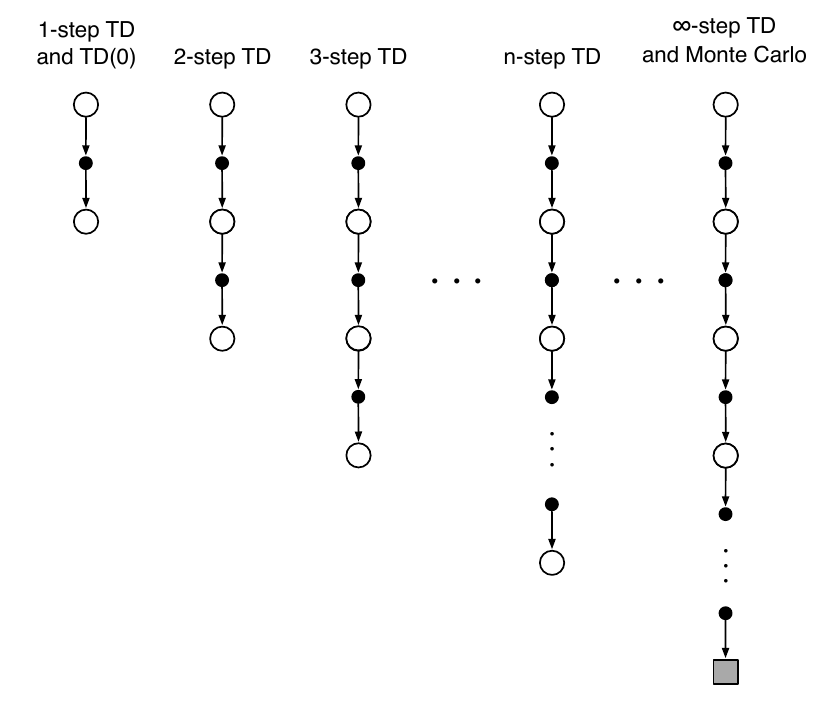
\includegraphics[width=0.3\textwidth]{figures/td_n_step.png}
\end{figure}

Consider the following $n$-step returns for $n=1,2, \dots, \infty$:
\begin{alignat*}{3}
    n &= 1      &\quad \textcolor{blue}{(TD)} &\quad G_t^{(1)}      &&= R_{t+1} + \gamma v(S_{t+1}) \\
    n &= 2      &\quad                        &\quad G_t^{(2)}      &&= R_{t+1} + \gamma R_{t+2} + \gamma^2 v(S_{t+2}) \\
      &\ \vdots &\quad \vdots                 &\quad                && \\
    n &= \infty &\quad \textcolor{blue}{(MC)} &\quad G_t^{(\infty)} &&= R_{t+1} + \gamma R_{t+2} + \dots + \gamma^{T-1} R_T
\end{alignat*}

So, in general, the $n$-step return is defined as:
\[
    G_t^{(n)} = R_{t+1} + \gamma R_{t+2} + \dots + \gamma^{n-1} R_{t+n} + \gamma^n V(S_{t+n})
\]

So, $n$-step TD learning can be calculated as:

\[
    V(S_t) \gets V(S_t) + \alpha \left( G_t^{(n)} - V(S_t) \right)
\]

\subsection{TD($\lambda$)}

Picking $n$ can be tough, and most certainly won't generalize to different environments, so let's find a way to avoid picking
altogether! We will do this by picking all different values of $n$ at once. How? The intuition is to average all the possible n-step returns into a single return. If we average these values in a smart way, we can do it super quick and still have something that intuitively makes sense.
Now we note that a valid update can be done not just toward any n-step return, but toward any average of n-step returns for different $n$-s. For example, an update can be done toward a target that is half of a two-step return and half of a four-step return: $\frac{1}{2}G_t^{(2)} + \frac{1}{2} G_t^{(4)}$.


\begin{figure}[htbp]
    \centering
    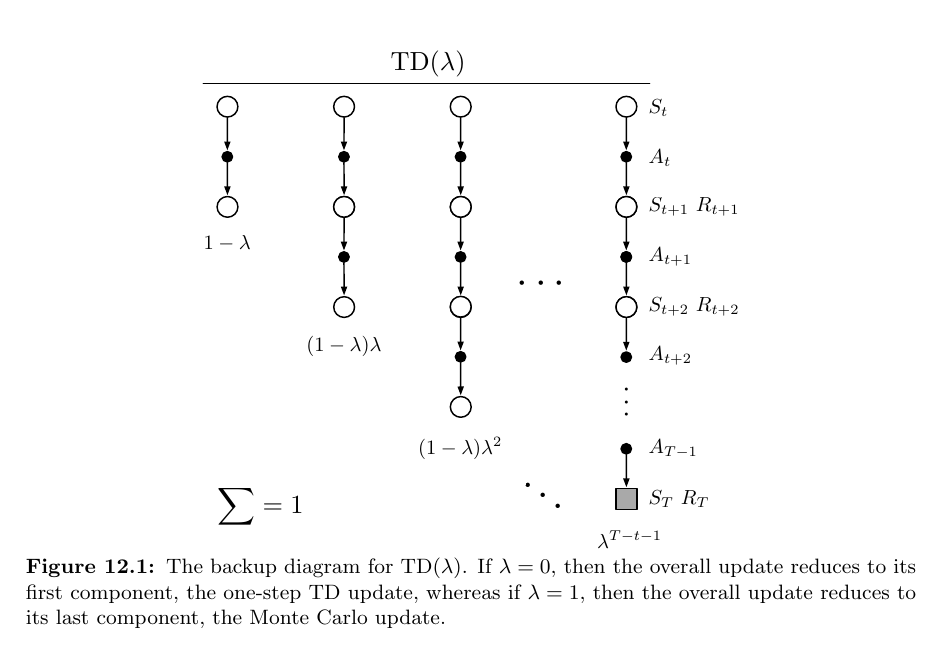
\includegraphics[width=0.5\textwidth]{figures/td_lambda.png}
\end{figure}

The $TD(\lambda)$ algorithm can be understood as one particular way of averaging $n$-step return $G_t^{(n)}$ using a weight that decays exponentially with time.  This average contains all the $n$-step updates, each weighted proportionally to $\lambda^{n-1}$ (where $\lambda \in [0, 1)$), and is normalized by a factor of $1-\lambda$ to ensure that the weights sum to 1. The resulting update is toward a return, called the $\lambda-return$, defined in its state-based form by:
\[
    G_t^\lambda \doteq (1-\lambda) \sum_{n=1}^{\infty} \lambda^{n-1} G_t^{(n)}
\]

The value function update for state $S_t$ then looks like a standard Monte Carlo update, but targeting $G_t^\lambda$:
$$V(S_t) \leftarrow V(S_t) + \alpha \left( G_t^\lambda - V(S_t) \right)$$

Note that to calculate $G_t^\lambda$ at time step $t$, you must wait until the episode finishes (or until far into the future) to collect $R_{t+1}, R_{t+2}, \dots, R_T$.

The approach that we have been taking so far is what we call the theoretical, or \emph{forward}, view of a learning algorithm. For each state visited, we look forward in time to all the future rewards and decide how best to combine them. We might imagine ourselves riding the stream of states, looking forward from each state to determine its update.

\begin{figure}[htbp]
    \centering
    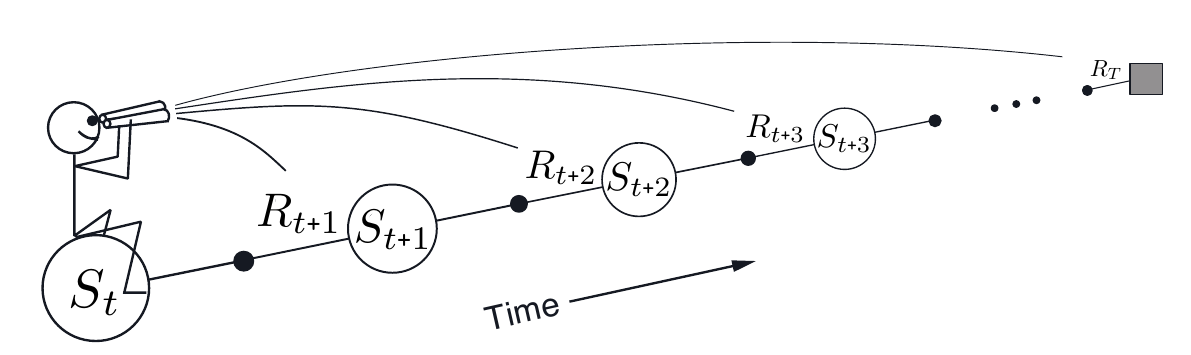
\includegraphics[width=0.5\textwidth]{figures/forward_view.png}
\end{figure}

After looking forward from and updating one state, we move on to the next and never have to work with the preceding state again. Future states, on the other hand, are viewed and processed repeatedly, once from each vantage point preceding them.

\subsection{Eligibility Traces}
We can clearly see that $TD(\lambda)$ with forward view has the same issues as Monte-Carlo: we have to wait until the episode ends to actually learn something. That's why \emph{backward} view was introduced: while forward view provides the theory, the backward view provides the actual mechanism used. But before going there we have to dive into the important concept of \textbf{eligibility traces}. Here, instead of waiting for what is going to happen next to be able to perform an update, we will remember what happened in the past and use current information to update the state-values for every state we've seen so far.

Let's start with a simple example: imagine you're a mouse going after a piece of cheese but, when you're nearing it, you hear a bell three times, a light comes on and you get electrocuted. Now: did the mouse get electrocuted because of the bell (most \emph{frequent} occurring state) or because of the light (most \emph{recent} occuring state)? Eligibility traces combine both the frequency and recency heuristics:
\begin{align*}
    E_0(s) &= 0 \\
    E_t(s) &= \gamma \lambda E_{t-1}(s) + \mathbbm{1}(S_t=s) \quad \forall \, s \in \mathcal{S}
\end{align*}

The idea is that every time we visit the state $S_t = s$ we increase the eligibility traces by adding $+1$. As we start not visiting that state anymore, the eligibility traces decay exponentially.

So now we can actually introduce the \emph{backward} view $TD(\lambda)$ algorithm: we keep an eligibility trace for every state $s$ then we update the value $V(s)$ for every state $s$ in proportion to the TD-error $\delta_t$ and eligibility trace $E_t(s)$:
\begin{align*}
    \delta_t &= R_{t+1} + \gamma V(S_{t+1}) - V(S_t) \\
    V(S) &\gets V(S) + \alpha \delta_t E_t(S)
\end{align*}

\begin{figure}[htbp]
    \centering
    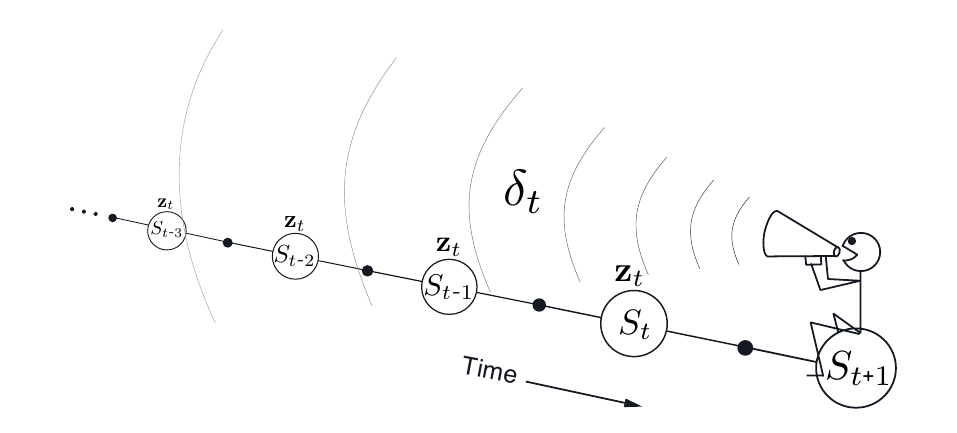
\includegraphics[width=0.5\textwidth]{figures/backward_view.png}
\end{figure}

So now we're no longer looking into the future, but instead we sort of "broadcast" this TD-error backwards to every state in the past, and the value function at each of those states is updated in proportion to the TD-error.

\paragraph{TD($\lambda$) and TD(0)}
When $\lambda = 0$, only the current state gets updated, so:
\begin{align*}
    E_t(s) &= \mathbbm{1}(S_t=s) \\
    V(s) &\gets V(s) + \alpha \delta_t E_t(s)
\end{align*}
Which is exactly equivalent to the TD(0) update $V(S_t) \gets V(S_t) + \alpha \delta_t$

\begin{table}[htbp]
    \centering
    \caption{Forward vs.\ Backward View of $\text{TD}(\lambda)$}
    \begin{tabularx}{\linewidth}{l X X}
    \toprule
     & \textbf{Forward view} & \textbf{Backward view} \\
    \midrule
    What it computes & $\lambda$-return $G_t^\lambda$ & Eligibility trace $E_t(s)$ \\
    \addlinespace
    When can you update? & Only at episode end & Every timestep \\
    \addlinespace
    Role & Theoretical target & Online mechanism \\
    \addlinespace
    Equiv.\ to TD(0) when & $\lambda = 0$ & $E_t(s) = \mathbbm{1}(S_t = s)$ \\
    \addlinespace
    Equiv.\ to MC when & $\lambda = 1$ & Trace decays only by $\gamma$, never by $\lambda$ \\
    \bottomrule
    \end{tabularx}
\end{table}


\section{Model-Free Control}
In this section we will see how to \emph{optimize} the value function of an \emph{unknown} MDP.

Before going into details, there's an important distinction we must make to understand everything that will come after:
\begin{itemize}
    \item \textbf{On-policy} learning: we have some policy $\pi$, we follow this policy, and we learn about it in the process
    \item \textbf{Off-policy} learning: we learn about a policy $\pi$ from experience sampled from an external policy $\mu$ (ex. learning from human behavior)
\end{itemize}

The main framework we are going to use is the same one we saw some sections ago, and that is \emph{policy iteration} in which we alternate two different processes:
\begin{itemize}
    \item \textbf{Policy evaluation:} where we estimate $v_\pi$ (e.g. iterative policy evaluation)
    \item \textbf{Policy improvement:} where we generate a new policy $\pi' \geq \pi$ (e.g. Greedy policy improvement)
\end{itemize}

The question now becomes the following: what can we slot in for these two processes? Firstly we can try to put in Monte-Carlo policy evaluation and $\epsilon$-greedy policy improvement.

\begin{figure}[htbp]
    \centering
    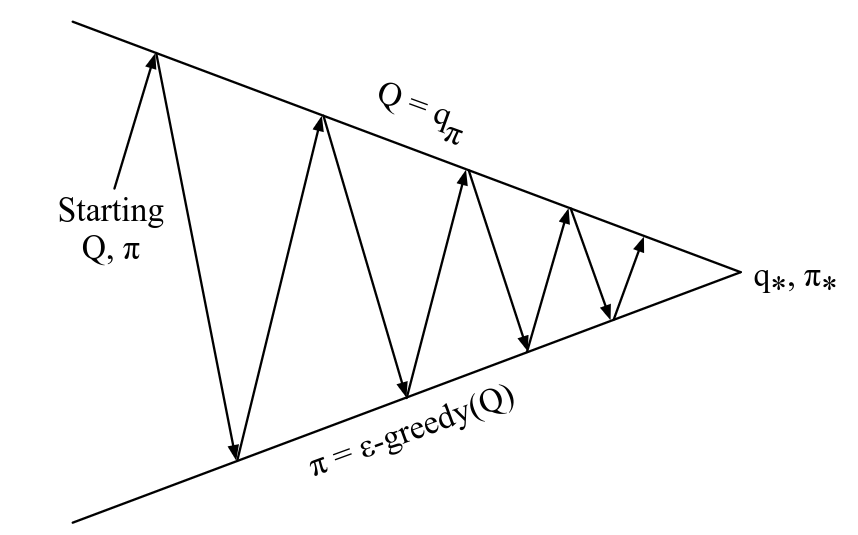
\includegraphics[width=0.5\textwidth]{figures/mc_policy_iteration.png}
\end{figure}

Here we use the $Q$ values because greedy policy improvement over $V$ requires the MDP:
\[
    \pi'(s) = \argmax_{a \in \mathcal{A}} \, \mathbb{E}[\underbrace{R_{t+1} + \gamma V(S_{t+1})}_{\text{Need to know next state}} \mid S_t = s, A_t = a]
\]

Meanwhile, with $Q(s,a)$ the greedy policy improvement becomes \textbf{model-free}:
\[
    \pi' = \argmax_{a \in \mathcal{A}} \, Q(s,a)
\]

Now let's try making this more efficient. We know from DP that in this policy iteration frameworks it is not necessary to go all the way to the top of the $Q=q_\pi$ line every time.

The idea here is to update $Q$ using only a few steps or a single episode, and then immediately update policy $\pi$ to be $\epsilon$-greedy with respect to the current $Q$. This is done because even a slightly better $Q$ gives us a better policy, and a better policy helps us collect better data to refine $Q$.

\begin{figure}[htbp]
    \centering
    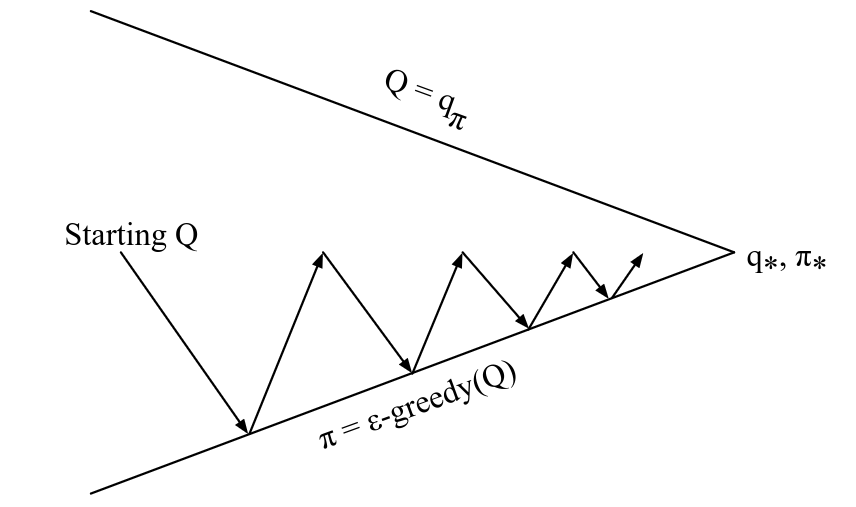
\includegraphics[width=0.5\textwidth]{figures/mc_control.png}
\end{figure}

Now a question comes up: can we guarantee that we will asintotically converge towards the optimal $q_\star$ and $\pi_\star$?

\paragraph{Greedy in the Limit with Infinite Exploration (GLIE)}

\begin{itemize}
    \item All state-action pairs are explored infinitely many times:
        \[ \lim_{k \to \infty} N_k(s,a) = \infty \]
    \item The policy converges on a greedy policy:
    \[
        \lim_{k \to \infty} \pi_k (a \mid s) = \mathbbm{1}(a = \argmax_{a' \in \mathcal{A}} \, Q_k(s,a'))
    \]
\end{itemize}

\paragraph{GLIE Monte-Carlo Control}
\begin{itemize}
    \item Sample $k$-th episode using our currently policy $\pi: \{ S_1, A_1, R_2, \dots, S_T \} \sim \pi$
    \item For each state $S_t$ and action $A_t$ in the episode:
    \begin{align*}
        N(S_t, A_t) &\gets N(S_t, A_t) + 1 \\
        Q(S_t, A_t) &\gets Q(S_t, A_t) + \frac{1}{N(S_t, A_t)}(G_t - Q(S_t, A_t))
    \end{align*}
    \item Improve policy based on new action-value function:
    \begin{align*}
        \epsilon &\gets 1/k \\
        \pi &\gets \epsilon\text{-greedy}(Q)
    \end{align*}
\end{itemize}

\begin{theorem}
    GLIE Monte-Carlo control converges to the optimal action-value function $$Q(s,a) \to q_\star(s,a)$$
\end{theorem}

\subsection{SARSA: On-policy TD Control}
We already know, in fact, that MC has several disadvantages when compared to TD (such as higher variance, being offline and having to complete the sequence to learn), so the natural idea becomes to substitute MC with TD in the control loop by:
\begin{itemize}
    \item Applying TD to $Q(S,A)$
    \item Use $\epsilon$-greedy policy improvement
    \item Update every time step
\end{itemize}

The name SARSA comes out because of how this algorithm works:
\begin{enumerate}
    \item We start from some state-action pair $(S_t, A_t)$
    \item We then randomly sample from the environment, get a reward $R_{t+1}$ and end up in some state $S_{t+1}$
    \item Then we sample our policy again to generate $A_{t+1}$ from $S_{t+1}$
\end{enumerate}

This rule uses every element of the quintuple of events, $(S_t, A_t , R_{t+1} , S_{t+1} , A_{t+1} )$, that make up a transition from one state-action pair to the next. 

SARSA mainly indicates a particular upgrade rule:
\[
    Q(S_t,A_t) \gets Q(S_t,A_t) + \alpha (R_{t+1} + \gamma Q(S_{t+1},A_{t+1}) - Q(S_t,A_t))
\]

\begin{algorithm}
    \caption{SARSA for On-Policy Control}
    \begin{algorithmic}[1]
        \State Initialize $Q(s,a)$ lookup table $\forall s \in \mathcal{S}, a \in \mathcal{A}$ arbitrarily
        \Repeat{ for each episode}
            \State Initialize $S$
            \State Choose $A$ from $S$ using policy derived from $Q$ (e.g. $\epsilon$-greedy)
            \For{\textbf{each} step of episode}
                \State Take action $A$ and observe $R,S'$
                \State Choose $A'$ from $S'$ using policy derived from $Q$
                \State $Q(S,A) \gets Q(S,A) + \alpha [R + \gamma Q(S',A') - Q(S,A)]$
                \State $S \gets S'$; $A \gets A'$;
            \EndFor
        \Until{$S$ is terminal}
    \end{algorithmic}
\end{algorithm}

\begin{theorem}
    SARSA converges to the optimal action-value function $Q(s,a) \to q_\star(s,a)$ under the following conditions:
    \begin{itemize}
        \item GLIE sequence of policies $\pi_t(a \mid s)$
        \item Robbins-Monro sequence of step-sizes $\alpha_t$:
        \begin{align*}
            \sum_{t=1}^{\infty} \alpha_t = \infty \\
            \sum_{t=1}^{\infty} \alpha_t^2 < \infty
        \end{align*}
        Step sizes must be sufficiently large that we can move $Q$ value as far as we want but eventually changes to $Q$ values vanish
    \end{itemize}
\end{theorem}

\subsection{Q-Learning: Off-Policy TD Control}
In off-policy learning we want to go ahead and evaluate the target policy $\pi(a \mid s)$ while following another behavior policy $\mu(a \mid s)$.

In this case, the learned action-value function, $Q$, directly approximates $q_\star$ , the optimal
action-value function, independent of the policy being followed.

\[
    Q(S_t, A_t) \gets Q(S_t, A_t) + \alpha \left[ R_{t+1} + \gamma \max_a Q(S_{t+1}, a) - Q(S_t, A_t) \right]
\]

Essentially we have the following situation:
\begin{itemize}
    \item The next action is chosen by using the behavior policy: $A_{t+1} \sim \mu(\cdot \mid S_{t+1})$ which, in Q-learning's case, is the $\epsilon$-greedy policy
    \item But we also consider an alternative successor action $A' \sim \pi(\cdot \mid S_{t+1})$ which, in Q-learning's case, is the \textbf{greedy policy}: $\pi(S_{t+1}) = \argmax_{a'} Q(S_{t+1}, a')$
\end{itemize}

What we want to do is to learn a greedy behavior, but we're following some exploratory behavior.

\begin{algorithm}
    \caption{Q-learning (Off-Policy TD Control)}
    \begin{algorithmic}[1]
        \State Initialize $Q(s,a)$ lookup table $\forall s \in \mathcal{S}^+, a \in \mathcal{A}(s)$ arbitrarily, except $Q(\text{terminal}, \cdot) = 0$
        \Repeat{ for each episode}
            \State Initialize $S$
            \For{\textbf{each} step of episode}
                \State Choose $A$ from $S$ using policy derived from $Q$ (e.g. $\epsilon$-greedy)
                \State Take action $A$ and observe $R, S'$
                \State $Q(S,A) \gets Q(S,A) + \alpha \left[ R + \gamma \max_{a} Q(S',a) - Q(S,A) \right]$
                \State $S \gets S'$
            \EndFor
        \Until{$S$ is terminal}
    \end{algorithmic}
\end{algorithm}

\subsubsection{Double Q-Learning}
In Q-learning the target policy is the greedy policy given the current action values, which is defined with a max. In this algorithm, a maximum over estimated values is used implicitly as an estimate of the
maximum value, which can lead to a significant positive bias. 

To better understand this let's use a roulette as an example. Imagine you walk into a casino and sit down at a table. You have two choices:
\begin{itemize}
    \item Choice A (Walk Away): You don't play. You get \$0
    \item Choice B (Play Roulette): You bet \$1 on one of the 36 betting options on the roulette wheel.
\end{itemize}
Because the house always has an edge, the true expected return for placing a roulette bet is slightly negative -- say, $-0.05$ on average, but because roulette is stochastic, you won't get $-0.05$ every single spin. It's natural that we will lose most of the time, but when we get lucky and win, we'll get a positive reward and Q-learning just cares about this max, and nothing else. Because the $\max$ operator always selects the luckiest outlier, Q-learning falls into the illusion that playing roulette is profitable. It will repeatedly choose to play roulette instead of walking away.

The root cause of maximization bias is using the same set of Q-values for both:
\begin{enumerate}
    \item Selecting which action is best ($\argmax_a$)\footnote{Recall that $\max_a Q(S_{t+1}, a) = Q(S_{t+1}, \argmax_a Q(S_{t+1},a))$}
    \item Evaluating the value of that action ($Q(s, a)$).
\end{enumerate}

In general: 
\[
    \mathbb{E}\big[\max_a Q_t(a)\big] \;\geq\; \max_a\, \mathbb{E}\big[Q_t(a)\big] = \max_a q_\star(a)
\]


Double Q-Learning solves this by decoupling action selection from action evaluation using two independent Q-tables ($Q_1$ and $Q_2$). With $p = 0.5$, update $Q_1$ using $Q_2$ for evaluation:

$$Q_1(S_t,A_t) \gets Q_1(S_t,A_t) + \alpha [R_{t+1} + \gamma Q_2(S_{t+1}, \argmax_a Q_1(S_{t+1},a)) - Q_1(S_t,A_t)]$$ 

and otherwise, symmetrically, update Q2 using Q1. The two tables take turns being "the selector" and "the judge," which is what prevents either one from ever grading its own optimistic homework.

We maintain two separate action-value functions, $Q_1(s, a)$ and $Q_2(s, a)$, trained on different subsets of experience (e.g., by randomly splitting incoming time steps) and, when updating:
\begin{itemize}
    \item We use $Q_1$ to \textbf{select} the best action $a^\star = \argmax_a Q_1(S_{t+1},a)$
    \item We use $Q_2$ to \textbf{evaluate} that action $Q_2(S_{t+1}, a^\star)$
\end{itemize}

Going back to the roulette example, Double Q-Learning fixes the maximization bias problem because:
\begin{itemize}
    \item $Q_1$ picks the winner: $Q_1$ looks at its data and picks the highest estimate: "Bet 3 looks best to me!"
    \item $Q_2$ evaluates that pick: Instead of trusting $Q_1$'s positive score, we look up Bet 3 in $Q_2$'s independent dataset.
\end{itemize}

In $Q_2$'s independent history, Bet 3 wasn't as lucky, so the reward turns out as negative.

$$\text{Double Q Target} = Q_2(\text{argmax } Q_1) = Q_2(\text{Bet 3}) = \textbf{Negative value} $$


\subsection{Importance Sampling Corrections}
Firstly we need to estimate the expectation of $f(X)$ under a different (target) distribution $P$:

\begin{align*}
    \mathbb{E}_{X \sim P}[f(X)] &= \sum P(X)f(X) \\
                                &= \sum Q(X) \frac{P(X)}{Q(X)}f(X) \\
                                &= \mathbb{E}_{X \sim Q}\left[ \frac{P(X)}{Q(X)}f(X) \right]
\end{align*}

\subsubsection{Importance Sampling for Off-Policy MC}
The goal is to estimate $v_\pi$ by using returns generated from the behavioral policy $\mu$ to evaluate $\pi$. The key insight is to weight the return $G_t$ according to the similarities between policies $\pi/\mu$:

\[
    G_t^{\pi/\mu} = \left( \frac{\pi(A_t \mid S_t)}{\mu(A_t \mid S_t)} \cdot \frac{\pi(A_{t+1} \mid S_{t+1})}{\mu(A_{t+1} \mid S_{t+1})} \cdot \dots \cdot \frac{\pi(A_T \mid S_T)}{\mu(A_T \mid S_T)} \right) \cdot G_t
\]

For every single step in the episode from $t$ to $T$, you multiply by the ratio:

$$\frac{\text{Probability of taking action } A_t \text{ under target policy } \pi}{\text{Probability of taking action } A_t \text{ under behavior policy } \mu}$$

When policy $\mu$ generates a trajectory, the actions it took might be very likely or unlikely under policy $\pi$. The ratio adjusts for this:

\begin{itemize}
    \item If $\pi(A\vert{}S) > \mu(A\vert{}S)$: policy $\pi$ would have taken this action much more often than $\mu$ did. Therefore, this episode's return $G_t$ was under-represented, so we up-weight it.
    \item If $\pi(A\vert{}S) < \mu(A\vert{}S)$: policy $\pi$ rarely takes this action compared to $\mu$. This return was over-represented, so we down-weight it.
    \item If $\pi(A\vert{}S) = 0$: Policy $\pi$ would never take this action. The entire return $G_t$ gets zeroed out because it's irrelevant to $\pi$.
\end{itemize}

Multiplying together $\pi(A_t|S_t)/\mu(A_t|S_t)$ across an entire episode means the correction weight is a product of ratios, one per timestep. Even if each ratio is well-behaved, the product's variance can grow exponentially with episode length. This is why full-return importance sampling is rarely used in practice for long episodes, and why the TD version in \ref{sec:importance_sampling_td} (which only needs a single step's ratio per update) is generally preferred. Note also that this only works if $\mu(a \mid s) > 0 $, otherwise we'd have $0$ in the denominator.

\subsubsection{Importance Sampling for Off-Policy TD}\label{sec:importance_sampling_td}
Here we use the TD targets generated from $\mu$ to evaluate $\pi$ and weigh them by importance sampling:

\[
    V(S_t) \gets V(S_t) + \alpha \left( \frac{\pi(A_t \vert S_t)}{\mu(A_t \vert S_t)}(R_{t+1} + \gamma V(S_{t+1})) - V(S_t) \right)
\]

\subsection{Expected SARSA}
Consider the learning algorithm that is just like Q-learning except that instead of the maximum over next state-action pairs it uses the expected value, taking into account how likely each action is under the current policy. That is, consider the algorithm with the update rule:

\begin{align*}
    Q(S_t, A_t) &\gets Q(S_t, A_t) + \alpha \left[ R_{t+1} + \gamma \mathbb{E}_\pi [Q(S_{t+1},A_{t+1}) \mid S_{t+1}] - Q(S_t, A_t) \right] \\
               &= Q(S_t, A_t) + \alpha \left[ R_{t+1} + \gamma  \sum_{a} \pi(a \mid S_{t+1})Q(S_{t+1},a) - Q(S_t, A_t) \right]
\end{align*}

Given the next state, $S_{t+1}$, this algorithm moves \emph{deterministically} towards the same direction as SARSA moves \emph{in expectation}, and accordingly it is called \emph{Expected SARSA}. Thus, expected SARSA eliminates the variance caused by random action selection ($A_{t+1}$). Note that the cost of this variance reduction is computational: the sum over all actions costs $\mathcal{O}(\lvert A \rvert)$ per step, versus $\mathcal{O}(1)$ for plain SARSA or Q-learning.

Expected SARSA can be both On- and Off-Policy:
\begin{itemize}
    \item If we take $\pi$ as the greedy policy ($\pi(a \mid S_{t+1}) = 1$ for the best action, $0$ otherwise), then Expected SARSA collapses into standard Q-learning.
\end{itemize}

\begin{table}[h]
    \centering
    \caption{On-Policy vs.\ Off-Policy Control Algorithms}
    \begin{tabularx}{\linewidth}{l l l X}
    \toprule
    \textbf{Algorithm} & \textbf{On/Off-policy} & \textbf{Update target} & \textbf{Notes} \\
    \midrule
    SARSA & On-policy & $R + \gamma Q(S',A')$, $A'$ & Learns the value of the $\epsilon$-greedy policy it runs \\
    \addlinespace
    Q-Learning & Off-policy & $R + \gamma \max_a Q(S',a)$ & Prone to maximization bias \\
    \addlinespace
    Double Q-Learning & Off-policy & $R + \gamma\, Q_2\!\left(S', \operatorname*{argmax}_a Q_1(S',a)\right)$ & Decouples selection from evaluation \\
    \addlinespace
    Expected SARSA & Either & $R + \gamma \sum_a \pi(a\mid S')Q(S',a)$ & Reduces to Q-learning if $\pi$ is greedy \\
    \addlinespace
    Off-policy MC (IS) & Off-policy & episode return weighted $\prod \pi/\mu$ & High variance \\
    \bottomrule
    \end{tabularx}
\end{table}

\section{Function Approximation}
Everything from DP through Q-learning assumed we could afford one table cell per state (or state-action pair). That assumption dies the moment states are continuous (robot joint angles, pixel images) or just combinatorially large (Backgammon has $\sim 10^20$ states) -- there isn't enough memory to store the table, let alone enough experience to fill every cell. Function approximation trades exactness for compactness: instead of memorizing a value per state, we learn a function with far fewer parameters than there are states, and rely on generalization to states we've never visited.

\begin{align*}
    \hat{v}(s,\mathbf{w}) &\approx v_\pi(s) \\
    \text{or }\hat{q}(s, a, \mathbf{w}) &\approx q_\pi(s,a)
\end{align*}

Where $\mathbf{w} \in \mathbb{R}^d$ (with $d \ll \lvert \mathcal{S}\rvert$) represents a \emph{weight vector} that will approximate the value function. This way we can fit a function for each state we will be visiting while also being able to generalize the states which have yet to be seen by querying our function approximator in those states.

Now a question arises: \emph{which} function approximator is to be chosen for RL tasks? From now on we will only consider \textbf{differentiable} function approximators, e.g.:
\begin{itemize}
    \item Linear combinations of features
    \item Neural Networks
    \item \dots
\end{itemize}

The main difference of RL when compared to standard supervised learning is that in practice we end up with a non-stationary (always changing), non-iid (e.g. where I am now is highly correlated to where I will be at the next step) sequence of value functions we're trying to estimate.

\subsection{Incremental Methods}\label{sec:incremental-methods}
\subsubsection{Gradient Descent}
We now develop in detail one class of learning methods for function approximation in value prediction, those based on stochastic gradient descent (SGD). SGD methods are among the most widely used of all function approximation methods and are particularly well suited to online reinforcement learning.

Let $J(\mathbf{w})$ be a differentiable function with parameter vector $\mathbf{w}$. We define the gradient of $J(\mathbf{w})$ with respect to $\mathbf{w}$ as:

\[
\nabla_{\mathbf{w}} J(\mathbf{w}) = 
\begin{pmatrix}
\frac{\partial J(\mathbf{w})}{\partial \mathbf{w}_1} \\
\vdots \\
\frac{\partial J(\mathbf{w})}{\partial \mathbf{w}_n}
\end{pmatrix}
\]

The goal now is to find the local minimum of $J(\mathbf{w})$ and move the parameter $\mathbf{w}$ in the direction of the negative gradient:
\[
    \Delta \mathbf{w} = - \frac{1}{2} \alpha \nabla_{\mathbf{w}} J(\mathbf{w})
\]

With $\alpha$ being the step-size parameter.

Let's now imagine that we have an oracle that tells us the correct value of the value function $v_\pi$; if we had this we could just minimize the MSE between the approximate value and the true function value:

\[
    J(\mathbf{w}) = \mathbb{E}_\pi \left[ (v_\pi(s) - \hat{v}(s,\mathbf{w}))^2 \right]
\]

Now, following the gradient descent, we have:

\begin{align*}
    \Delta \mathbf{w} &= - \frac{1}{2} \alpha \nabla_{\mathbf{w}} J(\mathbf{w}) \\
                      &= \alpha \mathbb{E}_\pi \left[ ( v_\pi(s) - \hat{v}(s, \mathbf{w}) ) \nabla_{\mathbf{w}} \hat{v}(s,\mathbf{w}) \right]
\end{align*}

Stochastic gradient descent \emph{samples} the gradient:

\[
    \Delta \mathbf{w} = \alpha \left( v_\pi(s) - \hat{v}(s, \mathbf{w}) \right) \nabla_{\mathbf{w}} \hat{v}(s, \mathbf{w})
\]

\subsubsection{Linear Methods}
One of the most important special cases of function approximation is that in which the approximate function, $\hat{v}(\cdot, \mathbf{w})$, is a linear function of the weight vector, $\mathbf{w}$. Corresponding to every state $s$, there is a real-valued vector $\mathbf{x}(s) \doteq (x_1(s), x_2(s), \dots, x_d(s))^\top$, with the same number of components as $\mathbf{w}$. Linear methods approximate the state-value function by the inner product between $\mathbf{w}$ and $\mathbf{x}(s)$:

\[
    \hat{v}(s, \mathbf{w}) \doteq \mathbf{w}^\top \mathbf{x}(s) \doteq \sum_{i=1}^{d} w_i x_i(s)
\]

In this case the approximate value function is said to be linear. The vector $\mathbf{x}(s)$ is called a \textbf{feature vector} representing each state $s$: each one of its components $x_i(s)$ is the value of a function $x_i : \mathcal{S} \to \mathbb{R}$.

The objective function is quadratic in parameters $\mathbf{w}$:

\[
    J(\mathbf{w}) = \mathbb{E}_\pi \left[ ( v_\pi(s) - \mathbf{x}(s)^\top \mathbf{w} )^2 \right]
\]

SGD converges on global optimum and its update rule is particularly simple:

\begin{align*}
    \nabla_{\mathbf{w}} \hat{v}(s,\mathbf{w}) &= \mathbf{x}(s) \\
    \Delta \mathbf{w} &= \alpha \left( v_\pi(s) - \hat{v}(s,\mathbf{w}) \right) \mathbf{x}(s) \\
    \text{Update} &= \text{step-size} \times \text{prediction error} \times \text{feature value}
\end{align*}

Up until now we've been cheating: we do not have an oracle that tells us the exact value of $v_\pi$, otherwise we wouldn't be here talking right now. In practice we substitute a target for $v_\pi(s)$:
\begin{itemize}
    \item For MC, the target is the return $G_t$
    \[ 
        \Delta \mathbf{w} = \alpha \left( G_t - \hat{v}(S_t, \mathbf{w})\right) \nabla_{\mathbf{w}} \hat{v}(S_t, \mathbf{w})
    \]
    Here the return $G_t$ is an \emph{unbiased}, noisy sample of the true value $v_\pi(S_t)$, so we can therefore apply supervised learning to "training data":
    \[
        \langle S_1, G_1 \rangle, \langle S_2, G_2 \rangle, \dots, \langle S_T, G_T \rangle
    \]

    For example, using linear MC policy evaluation:
    \begin{align*}
        \Delta \mathbf{w} &= \alpha \left( G_t - \hat{v}(S_t, \mathbf{w}) \right) \nabla_{\mathbf{w}} \hat{v}(S_t, \mathbf{w}) \\
        &= \alpha \left( G_t - \hat{v}(S_t, \mathbf{w}) \right) \nabla_{\mathbf{w}} ( \mathbf{w}^\top \mathbf{x}(S_t) ) \\
        &= \alpha \left( G_t - \hat{v}(S_t, \mathbf{w})\right)  \mathbf{x}(S_t) 
    \end{align*}

    \item For TD(0), the target is the TD target $R_{t+1} + \gamma \hat{v}(S_{t+1}, \mathbf{w})$
    \[
        \Delta \mathbf{w} = \alpha \left( R_{t+1} + \gamma \hat{v}(S_{t+1}, \mathbf{w}) \right) \nabla_{\mathbf{w}} \hat{v}(S_t, \mathbf{w})
    \]

    Here the TD-target $R_{t+1} + \gamma \hat{v}(S_{t+1}, \mathbf{w})$ is a \emph{biased} sample of true value $v_\pi(S_t)$, but we can still apply supervised learning to "training data":

    $$
    \langle S_1, R_2 + \gamma \hat{v}(S_2, \mathbf{w})\rangle, \langle S_2, R_3 + \gamma \hat{v}(S_3, \mathbf{w})\rangle, \dots, \langle S_{T-1}, R_T \rangle
    $$

    For example, using linear TD(0):
    $$
    \begin{aligned} 
        \Delta \mathbf{w} &= \alpha \left( R + \gamma \hat{v}(S', \mathbf{w}) - \hat{v}(S, \mathbf{w}) \right) \nabla_{\mathbf{w}} \hat{v}(S, \mathbf{w}) \\ &= \alpha \delta \mathbf{x}(S) 
    \end{aligned}
    $$
\end{itemize}

\subsection{Control with Value Function Approximation}
We are going to use the same idea for control as we already saw in the last section and build upon it by using \emph{approximate} policy evaluation $\hat{q}(\cdot, \cdot, \mathbf{w} \approx q_\pi)$

\begin{figure}[htbp]
    \centering
    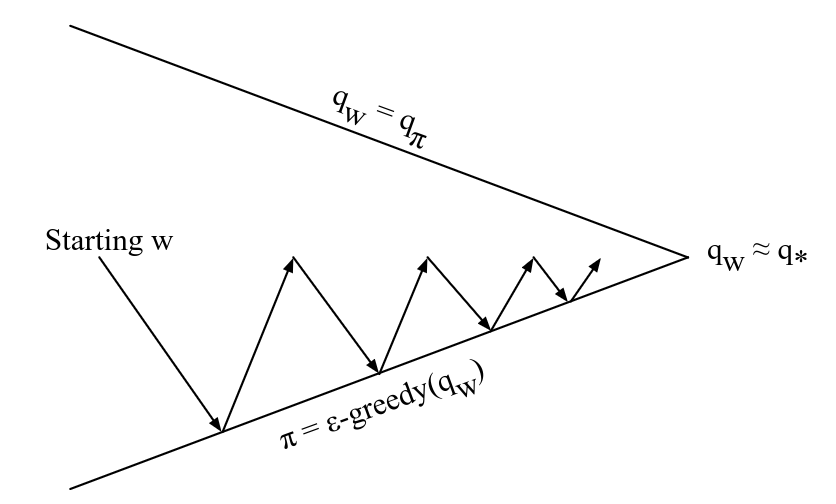
\includegraphics[width=0.5\textwidth]{figures/control_func_approx.png}
\end{figure}

As before we approximate the value function $\hat{q}(s,a,\mathbf{w}) \approx q_\pi(s,a)$ and minimize the MSE between approximate action-value function and true value action-value function:
\[
    J(\mathbf{w}) = \mathbb{E}\left[ (q_\pi(s,a) - \hat{q}(s,a,\mathbf{w}))^2 \right]
\]
And we use SGD to find a local minimum:

\begin{align*}
    -\frac{1}{2} \nabla_{\mathbf{w}} J(\mathbf{w}) &= \left( q_\pi(s,a) - \hat{q}(s,a,\mathbf{w}) \right) \nabla_{\mathbf{w}} \hat{q}(s,a,\mathbf{w}) \\
    \Delta \mathbf{w} &= \alpha \left( q_\pi(s,a) - \hat{q}(s,a,\mathbf{w}) \right) \nabla_{\mathbf{w}} \hat{q}(s,a,\mathbf{w})
\end{align*}

In general when dealing with continuous variables we cannot make a lookup table out of it since there are infinitely many states to deal with! So two possible solutions used in RL are the followings:
\begin{itemize}
    \item \textbf{Coarse Coding:} represents continuous states as binary features using overlapping circles, turning on features whenever a state falls inside them. Each cirle represents a single binary feature $x_i(s)$:
    \begin{itemize}
        \item If state $s$ lies in circle $i$ then $x_i(s) = 1$
        \item Else $x_i(s) = 0$
    \end{itemize}
    When a state $s$ is updated, the weights corresponding to all active circles update together. Any nearby state $s'$ that falls into the same overlapping circles instantly inherits that update-creating automatic, localized generalization.
    \item \textbf{Tile Coding:} is a fast, structured form of coarse coding that uses multiple uniform grid layers ("tilings") shifted slightly relative to each other, allowing linear models to generalize smoothly across continuous spaces.
\end{itemize}

\paragraph{Example: Mountain Car with Linear SARSA.}
The Mountain Car problem is a continuous control task where an underpowered car must reach a goal located at the top of a steep mountain slope on the right. Because gravity is stronger than the car's engine, applying full throttle from the valley is not enough to drive straight up the incline. To succeed, the agent must first take a counterintuitive action: driving in the opposite direction up the left slope to gather momentum, then using that built-up inertia along with full throttle to carry the car all the way up to the goal.

Here the reward is always $-1$ on all time steps until the car moves past the goal's position.

The feature vectors $\mathbf{x}(s,a)$ are created by tile coding and are then combined linearly with the parameter vector to approximate the action-value function.

\begin{figure}[htbp]
    \centering
    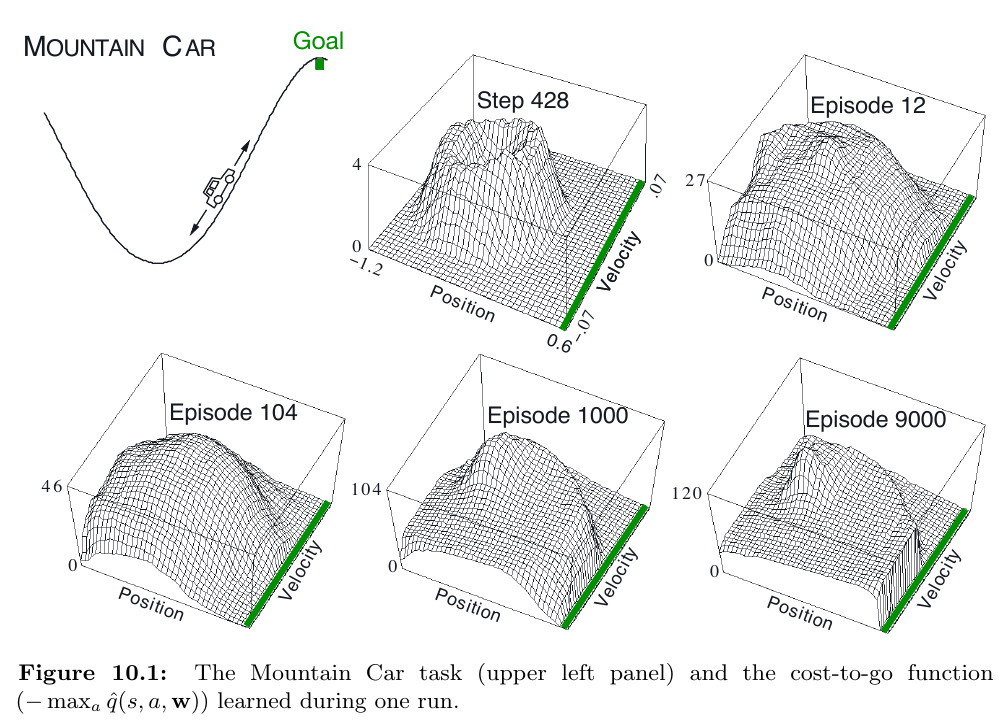
\includegraphics[width=0.5\textwidth]{figures/linear_sarsa_mountain_car.png}
\end{figure}

Shown is the negative of the value function (the \emph{cost- to-go} function) learned on a single run. The initial action values were all zero, which was optimistic (all true values are negative in this task), causing extensive exploration to occur even though the exploration parameter, $\varepsilon$, was 0. This can be seen in the middle-top panel of the figure, labeled “Step 428”. At this time not even one episode had been completed, but the car has oscillated back and forth in the valley, following circular trajectories in
state space. All the states visited frequently are valued worse than unexplored states, because the actual rewards have been worse than what was (unrealistically) expected. This continually drives the agent away from wherever it has been, to explore new states, until a solution is found.

\subsection{Algorithms Convergence}

\paragraph{Monte Carlo} With linear functions (and suitably decaying step sizes), MC converges to:
\begin{align*}
    \mathbf{w}_{\text{MC}} 
    &= \argmin_{\mathbf{w}} \mathbb{E}_\pi \!\left[ \left(G_t - v(S_t, \mathbf{w})\right)^2 \right] \\
    &= \argmin_{\mathbf{w}} \mathbb{E}_\pi \!\left[ \left(G_t - \mathbf{w}^\top \mathbf{x}_t\right)^2 \right] && \text{(using } v(S_t, \mathbf{w}) = \mathbf{w}^\top \mathbf{x}_t \text{)} \\
    &= \left( \mathbb{E}\left[ \mathbf{x}_t \mathbf{x}_t^\top \right] \right)^{-1} \mathbb{E}\left[ G_t \mathbf{x}_t \right]
\end{align*}

\paragraph{TD} With linear functions, TD converges to:
\[
    \mathbf{w}_{\text{TD}} = \left( \mathbb{E}\left[ \mathbf{x}_t \left(\mathbf{x}_t - \gamma \mathbf{x}_{t+1}\right)^\top \right] \right)^{-1} \mathbb{E}\left[ R_{t+1}\mathbf{x}_t \right]
\]

The TD update is not an actual \emph{gradient} update, but more of a \textbf{stochastic approximation} update (broader class than SGD):

\[
    \mathbf{w} \gets \mathbf{w} + \alpha ( \underbrace{R_{t+1} + \gamma \hat{v}(S_{t+1}, \mathbf{w})}_{\text{TD Target}} - \hat{v}(S_t, \mathbf{w}) ) \nabla_{\mathbf{w}} \hat{v}(S_t, \mathbf{w})
\]

It is not an actual gradient because, if we took the real gradient, we would get the following result:
$$\left( R_{t+1} + \gamma \hat{v}(S_{t+1}, \mathbf{w}) - \hat{v}(S_t, \mathbf{w}) \right) \left[ \mathbf{\color{red}{\gamma \nabla_{\mathbf{w}} \hat{v}(S_{t+1}, \mathbf{w})}} - \nabla_{\mathbf{w}} \hat{v}(S_t, \mathbf{w}) \right]$$

TD completely ignores the derivative of the target term ($\mathbf{\color{red}{\gamma \nabla_{\mathbf{w}} \hat{v}(S_{t+1}, \mathbf{w})}}$). It treats the TD target as if it was not dependent on $\mathbf{w}$: it takes into account the effect of changing the weight vector $\mathbf{w}$ on the estimate, but ignore its effect on the target. Because it only takes into account the effect of changing $\mathbf{w}$ on the estimate $\hat{v}(S_t, \mathbf{w})$, but ignores its effect on the target $\hat{v}(S_{t+1}, \mathbf{w})$, it is called a \emph{semi-gradient} method.

Because of this approximation TD does \textbf{not always converge}. When learning is on-policy with linear function approximation, the semi-gradient TD update happens to be stable because the stationary state distribution bounds the updates; however when we combine all three elements of the so-called \textbf{deadly triad}:
\begin{itemize}
    \item \textbf{Function Approximation:} scalable way of generalizing from a state space
    much larger than the memory and computational resources
    \item \textbf{Bootstrapping:} update targets that include existing estimates,  rather than relying exclusively on actual rewards and
    complete returns
    \item \textbf{Off-policy training:} training on a distribution of transitions other than that produced
    by the target policy. 
\end{itemize}

When $\mathbf{A}$ is not positive-definite, the semi-gradient update acts like an amplification feedback loop: updating $\mathbf{w}$ pushes the target $\hat{v}(S_{t+1}, \mathbf{w})$ even further away, causing the weight vector $\mathbf{w}$ to grow exponentially and diverge to $\pm \infty$.

Here $\mathbf{A} \coloneqq \mathbb{E}\big[\mathbf{x}_t(\mathbf{x}_t - \gamma \mathbf{x}_{t+1})^\top\big]$ is exactly the matrix inverted in the $\mathbf{w}_{TD}$ formula above: when it fails to be positive-definite, that inverse stops being a well-behaved contraction, which is the root cause of divergence.


\subsection{Batch Methods}
So far we have talked about gradient descent mechanisms: their updates are very simple, but they're not sample efficient. We see an experience once, we take an update adjusting the function approximation in the direction of that experience, and we move onto the next experience, throwing out the previous one: this is obviously not data-efficient. 

Batch method try to solve this issue by trying to find the best fitting value function to all the data we've seen in our batch (in this case, it's the agent's experience).

\subsubsection{Least Squares Temporal Difference (LSTD)}
The incremental TD updates from \ref{sec:incremental-methods} throw away each transition after a single small step. While this is memory-cheap it also is very sample-inefficient, and you also have to hand-tune a step size $\alpha$. LSTD's approach aims to solve directly for the $\mathbf{w}$ that best fits all the data you've collected, in one shot, with no step size to tune at all. The price is the $\mathcal{O}(n^2) - \mathcal{O}(n^3)$ cost per update instead of $\mathcal{O}(n)$, so it only makes sense when the feature dimension $d$ is small enough to afford it.

One way of finding this \emph{best fit} is to do it with the \emph{least squares} fit. Now if we want to fit our function approximator $\hat{v}(s, \mathbf{w}) \approx v_\pi(s)$ we can then define some dataset $\mathcal{D}$ consisting of $\langle \text{state}, \text{value}\rangle$ pairs:

\[
    \mathcal{D} = \{ \langle s_1, v_1^\pi \rangle, \langle s_2, v_2^\pi \rangle, \dots, \langle s_T v_T^\pi \rangle \}
\]

Assuming that the $v_i^\pi$ are some sort of oracle targets telling us the real value that $s_i$ should've had. Now which parameters \textbf{w} give the \emph{best fitting} value function $\hat{v}(s,\mathbf{w})$? \textbf{Least squares} algorithms find parameter vector \textbf{w} by minimizing the squared error between $\hat{v}(s_t, \mathbf{w})$ and target values $v_t^\pi$:

\begin{align*}
    \text{LS}(\mathbf{w}) &\doteq \sum_{t=1}^{T} (v_t^\pi - \hat{v}(s_t, \mathbf{w}))^2 \\
                          &= \mathbb{E}_{\mathcal{D}} [(v^\pi - \hat{v}(s,\mathbf{w}))^2]
\end{align*}

Now since $v_t^\pi$ is unknown, the best estimate for the value of state $s_t$ is the TD target:

\[
    R_{t+1} + \gamma \hat{v}(s_{t+1}, \mathbf{w})
\]

Recall that we already saw which parameters \textbf{w} gives us the best fitting for the value function:

\[
    \mathbf{w}_{\text{TD}} = \left( \mathbb{E}\left[ \mathbf{x}_t \left(\mathbf{x}_t - \gamma \mathbf{x}_{t+1}\right)^\top \right] \right)^{-1} \mathbb{E}\left[ R_{t+1}\mathbf{x}_t \right]
\]

So the idea is to use the closed-form equation's empirical loss:

\begin{align*}
    &\frac{1}{T} \sum_{t=1}^{T} \left( R_{t+1} + \gamma \hat{v}(s_{t+1}, \mathbf{w})  - \hat{v}(s_t, \mathbf{w}) \right) \mathbf{x}(s_t) \\
    &\Rightarrow \mathbf{w}_{\text{LSTD}} = \underbrace{\left( \sum_{t=1}^{T} \mathbf{x}(s_t) (\mathbf{x}(s_t) - \gamma \mathbf{x}(s_{t+1}))^\top \right)^{-1}}_{\mathbf{A}_t^{-1}} \underbrace{\left( \sum_{t=1}^{T} R_{t+1} \mathbf{x}(s_t) \right)}_{\mathbf{b}_t}
\end{align*}

We can update both $\mathbf{b}_t$ and $\mathbf{A}_t^{-1}$ incrementally online:
\begin{itemize}
    \item \textbf{Naive approach} ($\mathcal{O}(n^3)$):
    \[
        \mathbf{A}_{t+1} = \mathbf{A}_t + \mathbf{x}_t (\mathbf{x}_t - \gamma \mathbf{x}_{t+1})^\top \qquad \mathbf{b}_{t+1} = \mathbf{b}_t + R_{t+1} \mathbf{x}_t
    \]

    \item \textbf{Faster approach} ($\mathcal{O}(n^2)$):
    \begin{align*}
        \mathbf{A}_{t}^{-1} &= \mathbf{A}_{t-1}^{-1} - \frac{\mathbf{A}_{t-1}^{-1} \mathbf{x}_{t-1} (\mathbf{x}_{t-1} - \gamma \mathbf{x}_{t})^\top \mathbf{A}_{t-1}^{-1}}{1 + (\mathbf{x}_{t-1} - \gamma \mathbf{x}_{t})^\top \mathbf{A}_{t-1}^{-1} \mathbf{x}_{t-1}} \\
        \mathbf{b}_{t+1} &= \mathbf{b}_t + R_{t+1} \mathbf{x}_{t+1}
    \end{align*}
\end{itemize}

Where $\mathbf{x}_t \equiv \mathbf{x}(s_t)$.

\subsubsection{Experience Replay}
Here we make the dataset $\mathcal{D}$ an explicitly stored object (a replay buffer) containing past transitions $\langle S_t, A_t, R_t, S_{t+1} \rangle$. All we have to do now is sample transitions from this dataset $\langle S_t, A_t, R_t, S_{t+1} \rangle \sim \mathcal{D}$ and apply the semi-gradient update to $\mathbf{w}$ using the bootstrapped target $R_{t+1} + \gamma \hat{v}(S_{t+1}, \mathbf{w})$:

Here we make the dataset $\mathcal{D}$ an explicitly stored object (a replay buffer) containing past transitions $\langle S_t, A_t, R_t, S_{t+1} \rangle$. All we have to do now is sample transitions from this dataset $\langle S_t, A_t, R_t, S_{t+1} \rangle \sim \mathcal{D}$ and apply the semi-gradient update to $\mathbf{w}$ using the bootstrapped target $R_{t+1} + \gamma \hat{v}(S_{t+1}, \mathbf{w})$:

\[
    \Delta \mathbf{w} = \alpha \left( R_{t+1} + \gamma \hat{v}(S_{t+1}, \mathbf{w}) - \hat{v}(S_t, \mathbf{w}) \right) \nabla_{\mathbf{w}} \hat{v}(S_t, \mathbf{w})
\]

This converges to the least squares solution $\mathbf{w}^\pi = \argmin_\mathbf{w} \text{LS}(\mathbf{w})$

\section{Deep Reinforcement Learning}
\subsection{Deep Value Function Approximation \& Automatic Differentiation}
In high-dimensional or continuous state spaces, linear value function approximation is insufficient to capture complex, non-linear relationships. Instead, Deep Neural Networks (DNNs) are used to parameterize value functions $v(s, \mathbf{w})$ or action-value functions $q(s, a, \mathbf{w})$.

\paragraph{Parameterization via Deep Networks.} A Multi-Layer Perceptron (MLP) calculates state values through sequential non-linear transformations:
$$v(S, \mathbf{w}) = \mathbf{W}_2 \tanh(\mathbf{W}_1 \cdot S + \mathbf{b}_1) + \mathbf{b}_2$$

where $\mathbf{w} = \{\mathbf{W}_1, \mathbf{b}_1, \mathbf{W}_2, \mathbf{b}_2\}$ represents the trainable weights and biases of the network.

\paragraph{Computational Graphs and Automatic Differentiation} Unlike linear function approximation (where gradients $\nabla_\mathbf{w} v(\cdot, \mathbf{w})$ are trivial to compute), deep architectures rely on computational graphs:
\begin{itemize}
    \item Computational Graph: Defines the sequence of operations as a Directed Acyclic Graph (DAG).
    \item Automatic Differentiation (Autodiff): Computes gradients of any output node with respect to any input parameter in a single backward sweep by applying the chain rule, accumulating products along paths, and summing gradients where paths merge.
\end{itemize}

\subsection{Deep Q-Learning (DQN)}
Deep Q-Learning parameterizes the action-value function $q_\mathbf{w}: \mathcal{S} \to \mathbb{R}^m$, mapping an input state $S_t$ to a vector of Q-values across $m$ discrete actions. 

\paragraph{Stabilizing Bootstrapping: Target Networks \& Experience Replay}
Standard Q-learning updates parameter vector $\mathbf{w}$ toward a bootstrapped target $Y_t = R_{t+1} + \gamma \max_{a} q(S_{t+1}, a, \mathbf{w})$. However, using the same weights $\mathbf{w}$ to compute both the prediction and the target causes severe instability: updating $\mathbf{w}$ to increase $q(S_t, A_t, \mathbf{w})$ simultaneously alters the target values for neighboring states, creating a moving target problem.

To resolve this, Deep Q-Networks (DQN) maintain two distinct networks:
\begin{enumerate}
    \item \textbf{Online Network ($q_\mathbf{w}$):} active parameters $\mathbf{w}$ that are continuously updated via gradient descent to select and evaluate actions.
    \item \textbf{Target Network ($q_{\mathbf{w}^-}$):} a semi-static copy with parameters $\mathbf{w}^-$, used exclusively to generate target labels $Y_t$. These parameters are periodically synchronized ($\mathbf{w}^- \leftarrow \mathbf{w}$) or softly updated every $C$ steps.
\end{enumerate}

Additionally, transitions $(S_t, A_t, R_{t+1}, S_{t+1})$ are stored in a replay buffer $\mathcal{D}$. Mini-batches of transitions are sampled uniformly to break temporal correlations between consecutive observations during optimization.

\paragraph{Loss Formulation}
The parameter update is framed as minimizing a Mean Squared Error (MSE) pseudo-loss over mini-batches sampled from $\mathcal{D}$:

$$L(\mathbf{w}) = \mathbb{E}_{(S_t, A_t, R_{t+1}, S_{t+1}) \sim \mathcal{D}} \left[ \frac{1}{2} \left( Y_t - q(S_t, A_t, \mathbf{w}) \right)^2 \right]$$

$$\text{where } Y_t = R_{t+1} + \gamma \max_{a} q\left(S_{t+1}, a, \mathbf{w}^-\right)$$

Because $Y_t$ is generated by the frozen target parameters $\mathbf{w}^-$, it acts as a fixed regression target during the update step. In automatic differentiation frameworks (e.g., JAX or PyTorch), this fixed-target treatment is enforced either by utilizing dedicated target network parameters or by applying a stop-gradient operator (\texttt{jax.lax.stop\_gradient}). Differentiating $L(\mathbf{w})$ with respect to $\mathbf{w}$ yields the desired semi-gradient update:

$$\nabla_{\mathbf{w}} L(\mathbf{w}) = - \mathbb{E}_{\mathcal{D}} \left[ \left( Y_t - q(S_t, A_t, \mathbf{w}) \right) \nabla_{\mathbf{w}} q(S_t, A_t, \mathbf{w}) \right]$$

\begin{figure}[htbp]
    \centering
    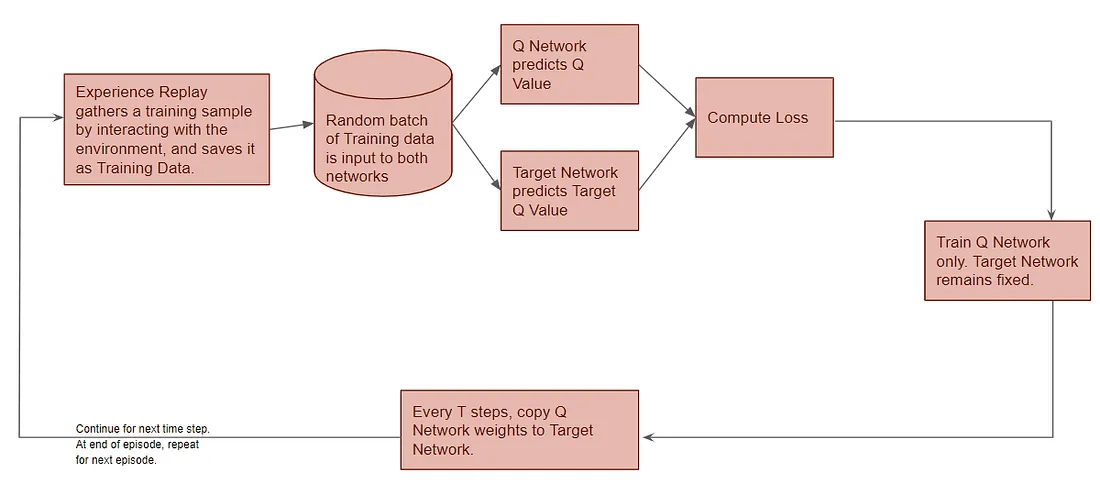
\includegraphics[width=0.70\textwidth]{figures/deep_q_learning.png}
\end{figure}

\subsection{Online Deep RL Issues \& Experience Replay}
Standard Deep Learning SGD optimization relies on the assumption that training data samples are independent and identically distributed (i.i.d.). Standard online RL violates this assumption:

\begin{itemize}
    \item \textbf{Online RL Bottleneck:} updates are performed on every step of sequential trajectories, resulting in highly correlated consecutive samples.
    \item \textbf{Experience Replay Solution:} stores historical transitions $(S_t, A_t, R_{t+1}, S_{t+1})$ in a buffer. Sampling mini-batches uniformly from the buffer:
    \begin{enumerate}
        \item Reduces correlation between consecutive updates.
        \item Enables stable mini-batch SGD updates instead of single-sample SGD.
    \end{enumerate}
    \item \textbf{Alternative Online Solutions:} Eligibility traces, momentum-based optimizers, and parallel environment execution.
\end{itemize}

\subsection{The Deadly Triad in Deep RL}
The Deadly Triad refers to the severe risk of divergence and instability arising when combining three core components:
\begin{enumerate}
    \item \textbf{Function Approximation:} fitting action values via neural networks
    \item \textbf{Bootstrapping:} target evaluation relying on estimated values
    \item \textbf{Off-Policy Learning:} learning from data collected under past/mixed policies
\end{enumerate}

\paragraph{Soft-Divergence}
In practical Deep RL settings, unbounded divergence is rare. Instead, algorithms suffer from soft-divergence -- transient value explosions that eventually recover after long training periods, severely degrading learning performance.

\subsection{RL-Aware Deep Learning Architectures \& Dynamics}
Rather than copying supervised learning architectures (e.g., standard CNNs/LSTMs), Deep RL benefits from structural inductive biases specifically designed for reinforcement learning dynamics.

\paragraph{Dueling Network Architecture} Decomposes action-value estimation into state-value and advantage streams:

$$q(s, a, \mathbf{w}) = v_\xi(s) + A_\chi(s, a) \quad \text{where } \mathbf{w} = \xi \cup \chi$$
\begin{itemize}
    \item $v_\xi(s)$: Represents how good it is to be in state $s$.
    \item $A_\chi(s, a)$: Represents the relative advantage of taking action $a$ over other actions.
\end{itemize}

\begin{figure}
    \centering
    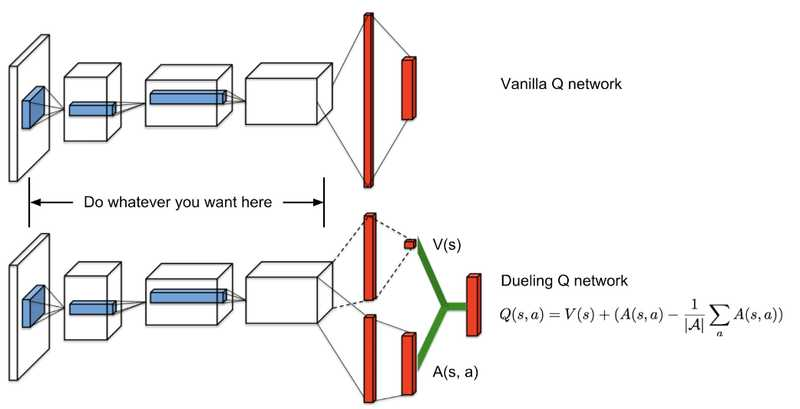
\includegraphics[width=0.65\textwidth]{figures/dueling-network-architectures.jpeg}
    \caption{Comparison between a standard DQN architecture (top) and a Dueling Q-network architecture (bottom). Both networks share identical convolutional feature-extraction layers. While vanilla DQN directly outputs action values $Q(s,a)$ from a single fully connected layer, the Dueling architecture splits into two separate streams to estimate state value $V(s)$ and action advantages $A(s,a)$, combining them via $Q(s,a) = V(s) + \left( A(s,a) - \frac{1}{|\mathcal{A}|}\sum_{a'} A(s,a') \right)$.}
    \label{fig:dueling_architecture}
\end{figure}

\textbf{Network Capacity \& Generalization Challenges}

\begin{itemize}
    \item \textbf{Capacity vs. Stability:} while increasing network size in supervised learning generally improves performance, larger networks in Deep RL are more susceptible to deadly triad instabilities despite achieving better final capacity.
    \item \textbf{Leakage Propagation:} combining Temporal Difference (TD) learning with deep function approximation leads to "leakage propagation," where approximation errors near sharp state-value discontinuities bleed into distant state regions. Monte Carlo methods do not suffer from leakage propagation.
    \item \textbf{Auxiliary Representation Learning:} to build representations resilient to improper generalization, state representations can be shared across auxiliary tasks—such as predicting values of multiple policies, predicting future observation frames, or controlling distinct auxiliary rewards (cumulants).
\end{itemize}

\end{document}
